\documentclass[11pt]{article}
\usepackage[margin=1in]{geometry}
\usepackage{amsmath,amssymb,amsthm}
\usepackage{xcolor}
\usepackage{tikz}
\usetikzlibrary{arrows.meta}
\usepackage{graphicx}
\usepackage[colorlinks=true,linkcolor=blue!60!black,citecolor=blue!60!black,urlcolor=blue!60!black]{hyperref}
\newcommand{\aside}[1]{\textcolor{blue}{#1}}
\newcommand{\Li}{\operatorname{Li}_2}
\newcommand{\atan}{\operatorname{arctan}}
\newcommand{\asinh}{\operatorname{arcsinh}}
\newcommand{\dd}{\,\mathrm{d}}
\newcommand{\nA}{\hat n_A}
\newcommand{\nB}{\hat n_B}
\newcommand{\Acap}{A^{\sigma}_{\cap}}
\title{The softened-log (Plummer) overlap:\\ a fully analytic mollification}
\author{}
\date{}

\begin{document}
\maketitle

\begin{abstract}
\noindent The Gaussian mollification of the polygon--polygon overlap area
(\texttt{smoothOverlap.tex}) is $C^\infty$ but forces Gauss--Legendre quadrature on
\emph{both} boundaries, because its potential has no elementary segment integral.
Replacing the Gaussian mollifier by the softened-log (Plummer) kernel preserves the
smoothness while making every boundary integral tractable in closed form.  This note
develops the model in three tiers of increasing analyticity: (i)~the exact reduction of
the mollified overlap and its shape gradient to double boundary integrals; (ii)~the
closed-form \emph{inner} panel integrals, which remove one quadrature loop
($\mathcal O(G^2)\!\to\!\mathcal O(G)$ per edge pair, implemented, $11\times$ faster);
and (iii)~--- new here --- the closed-form \emph{outer} integrals, which remove the last
quadrature ($\mathcal O(G)\!\to\!\mathcal O(1)$).  The final formulas are elementary
functions of the four corner--corner softened distances and angles, plus a single
transcendental object $\mathcal T$ built from four complex dilogarithms per edge pair
and per endpoint; the same $\mathcal T$ serves the energy and the vertex forces, and
the Plummer self-repulsion energy needs no dilogarithms at all.  Companion sections
treat the operational envelope: quantitative tail size and smooth truncation, kernel
selection (rational vs.\ compactly supported), the sharp $\sigma\to0$ limit and its
non-uniformities, and a reusable neighbor-list scheme reducing the global cost from
$\Theta(N^2E^2)$ to $\Theta(NzE^2)$ gates plus $\Theta(Nz\,E_{\text{act}})$
closed-form evaluations.  Every formula below
has been verified against adaptive quadrature at 25-digit working precision
(\texttt{verify\_plummer\_analytic.py}); \aside{blue text marks implementation status
and asides.}
\end{abstract}

\tableofcontents

%======================================================================
\section{Overview: why mollify, and the three-tier cost ladder}
%======================================================================

The sharp pair energy of the deformable-polygon model is built on the exact overlap
area $A_\cap = \int_{\mathbb R^2} \mathbf 1_A\,\mathbf 1_B\,\dd^2x$ of two polygons
$A,B$.  Exact overlap is piecewise analytic in the vertex positions: its gradient
jumps whenever a vertex crosses an edge of the partner, i.e.\ exactly at contact
formation and breaking.  Line-search minimizers tolerate this poorly close to a
minimum --- \aside{sharp CG launched from a well-relaxed configuration hard-stalls at
$\max|F|\approx 3.6\times10^{-3}$} --- because the energy landscape is only $C^0$
across the contact set.  Mollifying one indicator,
\begin{equation}
  \Acap \;=\; \int_{\mathbb R^2} \mathbf 1_A\,\bigl(K_\sigma * \mathbf 1_B\bigr)\,\dd^2x
  \;=\; \int_{\mathbb R^2}\!\!\int_{\mathbb R^2}
        \mathbf 1_A(\vec x)\,K_\sigma(\vec x-\vec x')\,\mathbf 1_B(\vec x')\,
        \dd^2x\,\dd^2x' ,
  \label{eq:defA}
\end{equation}
with a normalized $C^\infty$ kernel $K_\sigma$ of width $\sigma$ produces an energy
that is $C^\infty$ in all vertex coordinates and converges to $A_\cap$ as
$\sigma\to0$ \cite{Friedrichs1944,Evans2010}.  The second form of \eqref{eq:defA}
shows the construction is symmetric in $A\leftrightarrow B$ despite mollifying only
one factor: it is a proximity-weighted count of point pairs, one point in each body.

The computational question is what \eqref{eq:defA} costs.  Two divergence-theorem
reductions (\S\ref{sec:reductions}) convert the double area integral into a double
\emph{boundary} integral over edge pairs.  For the Gaussian kernel neither boundary
integral is elementary, so each of the $E_A E_B$ edge pairs costs a $G\times G$ tensor
quadrature.  The Plummer kernel of \S\ref{sec:kernel} makes the inner integral closed
form (\S\ref{sec:inner}), leaving a single smooth outer integral --- the
\emph{semi-analytic} tier, implemented in \texttt{plummerOverlap.py}.
\aside{On the $N=6$ packing this runs at 93\,ms per energy+gradient call at outer
$G=32$, versus 1040\,ms for the Gaussian version: $11\times$, with
force$\,=\nabla$energy to $\sim10^{-9}$.}  Section~\ref{sec:outer} completes the
program: the outer integral also closes, in elementary functions plus dilogarithms,
the standard transcendental level for Galerkin double integrations of logarithmic
kernels \cite{Salvadori2002,Carini1999,SauterSchwab2011}.  The ladder is
\[
  \underbrace{\mathcal O(G^2)}_{\text{Gaussian}}
  \;\longrightarrow\;
  \underbrace{\mathcal O(G)}_{\text{Plummer, semi-analytic}}
  \;\longrightarrow\;
  \underbrace{\mathcal O(1)}_{\text{Plummer, fully analytic}}
\]
per edge pair.  Beyond the constant-factor speedup, the fully analytic tier decouples
accuracy from geometry: the semi-analytic outer rule must resolve the
$\mathcal O(\sigma)$-scale variation of the integrand where $\partial A$ crosses
$\partial B$, so shrinking $\sigma$ forces $G$ up; the closed form is exact at any
$\sigma$.  Sections \ref{sec:sharplimit} and \ref{sec:neighbors} treat the two
remaining axes of cost and fidelity: the $\sigma\to0$ limit, and the global pair
count.

\paragraph{Context and roadmap.}  The setting is deformable-particle jamming
\cite{Boromand2018}: each grain is a polygon whose vertices are the degrees of
freedom, and the energy sums a shape-holding term (edge and area springs) with the
pairwise overlap penalty.  Relaxing to mechanical equilibrium and then probing stress
and stiffness demands an energy that is both smooth and minimizable to machine
precision --- neither of which the sharp overlap offers near the jammed contacts, which
sit exactly on its $C^0$ ridge.  The mollification \eqref{eq:defA} buys smoothness at a
fixed, controllable bias $\mathcal O(\sigma^2)$ (\S\ref{sec:tail}), and the reductions
below buy speed.  The plan: \S\ref{sec:kernel} fixes the kernel and its two potentials;
\S\ref{sec:reductions} runs the two divergence-theorem reductions to boundary
integrals; \S\S\ref{sec:winding}--\ref{sec:inner} evaluate the inner integrals in
closed form (semi-analytic tier); \S\ref{sec:outer} closes the outer integrals (fully
analytic tier, the technical heart); and \S\S\ref{sec:tail}--\ref{sec:neighbors} treat
tail, truncation, kernel choice, the sharp limit, and the neighbor list.  A reader who
only wants to \emph{use} the result can take
\eqref{eq:Iassembled}--\eqref{eq:Atotal} for the energy and
\eqref{eq:Wclosed}--\eqref{eq:deposit} for the force, with the primitives of
\S\S\ref{sec:masters}--\ref{sec:T}.

%======================================================================
\section{Kernel, potentials, and the softened step}
\label{sec:kernel}
%======================================================================

The mollifier is the two-dimensional Plummer (softened point-source) density
\begin{equation}
  K_\sigma(\vec r) \;=\; \frac{\sigma^2}{\pi\,\bigl(|\vec r|^2+\sigma^2\bigr)^{2}},
  \qquad \int_{\mathbb R^2} K_\sigma \,\dd^2 r = 1 ,
  \label{eq:kernel}
\end{equation}
a normalized, radially symmetric, $C^\infty$ bump of width $\sigma$ that tends to
$\delta^2(\vec r)$ as $\sigma\to0$.  It is the planar analogue of Plummer's stellar
density profile \cite{Plummer1911} and of the softened point mass of collisionless
$N$-body dynamics \cite{Aarseth1963}; in vortex methods the associated velocity field
is exactly Krasny's algebraically desingularized Biot--Savart kernel
\cite{Chorin1973,Krasny1986}, and in the blob-kernel classification of Beale and
Majda it is the lowest-order rational blob \cite{BealeMajda1985}.

The boundary reductions of \S\ref{sec:reductions} require a vector field $\vec F$
with $\nabla\!\cdot\!\vec F = K_\sigma$ and a scalar $\Phi$ with $\nabla\Phi=\vec F$.
By radial symmetry $\vec F = f(r)\,\hat r$ with $\frac1r (rf)' = K_\sigma$, so
\[
  f(r) \;=\; \frac1r\int_0^r r' K_\sigma(r')\,\dd r'
        \;=\; \frac{\sigma^2}{\pi r}\cdot\frac12\Bigl[\frac1{\sigma^2}
              -\frac1{r^2+\sigma^2}\Bigr]
        \;=\; \frac{r}{2\pi\,(r^2+\sigma^2)} ,
\]
and integrating once more,
\begin{equation}
  \vec F(\vec r) \;=\; \frac{\vec r}{2\pi\,(|\vec r|^2+\sigma^2)},
  \qquad
  \Phi(r) \;=\; \frac{1}{4\pi}\,\ln\!\bigl(r^2+\sigma^2\bigr).
  \label{eq:FPhi}
\end{equation}
$\vec F$ is rational and $\Phi$ a \emph{softened logarithm} --- no $\exp$, $\operatorname{erf}$
or $E_1$ anywhere, which is the entire point.  Both are the point-source pair
$\vec r/2\pi r^2$, $\tfrac1{2\pi}\ln r$ with the singularity rounded off, and both are
smooth at $r=0$; in particular self-panels and touching panels are perfectly regular,
so no singular-quadrature machinery is ever needed.  Geometrically $\vec F$ is the
softened Coulomb field of a unit 2D source: far out it is the bare $\vec r/2\pi r^2$
that a point source produces, while within $\sim\sigma$ the $r^2+\sigma^2$ denominator
turns the $1/r$ blow-up into the linear $\vec r/2\pi\sigma^2$ that vanishes at the
origin.  Every boundary integral below is finite precisely because its integrand never
sees the point-source singularity --- the price the Gaussian pays with $\exp$ and $E_1$,
the Plummer kernel pays with a single extra power in a denominator.

A closed form worth recording is the response to a half-plane.  The one-dimensional
marginal of \eqref{eq:kernel} is
$k_1(x)=\int K_\sigma(x,y)\,\dd y = \sigma^2/\bigl(2(x^2+\sigma^2)^{3/2}\bigr)$, so
the mollified indicator of a half-plane at signed distance $d$ from its boundary is
\begin{equation}
  s(d) \;=\; \int_{-d}^{\infty} k_1
       \;=\; \frac12\Bigl(1+\frac{d}{\sqrt{d^2+\sigma^2}}\Bigr):
  \label{eq:step}
\end{equation}
an \emph{algebraic sigmoid}.  The marginal itself is elementary:
$k_1(x)=\tfrac{\sigma^2}{\pi}\int_{-\infty}^{\infty}\dd y/(x^2+y^2+\sigma^2)^2
=\tfrac{\sigma^2}{\pi}\cdot\tfrac{\pi}{2(x^2+\sigma^2)^{3/2}}$ using the standard
$\int\dd y/(A^2+y^2)^2=\pi/2A^3$; integrating from the boundary,
$\int_{-d}^{\infty}(x^2+\sigma^2)^{-3/2}\dd x=\bigl[x/(\sigma^2\sqrt{x^2+\sigma^2})\bigr]_{-d}^{\infty}$,
gives \eqref{eq:step}.  Equation \eqref{eq:step} is what the whole construction
looks like from one meter away --- every sharp indicator in the theory is replaced by
this soft step evaluated on a suitable signed distance --- and it is odd about its
midpoint, $s(d)+s(-d)=1$, which controls the mollification bias
(\S\ref{sec:tail}).

The price of an algebraic kernel is the tail.  $K_\sigma\sim\sigma^2/\pi r^4$, so
two far, non-overlapping bodies carry a spurious overlap
$\Acap\approx \sigma^2 A_A A_B/(\pi r^4)$ that vanishes as $\sigma\to0$ but forbids a
hard distance cutoff (a cutoff would reintroduce a discontinuity, defeating the
construction).  \S\ref{sec:tail} quantifies this and sketches faster-decaying rational
kernels for which the same analytic program goes through.

%======================================================================
\section{Exact boundary reductions}
\label{sec:reductions}
%======================================================================

Two applications of the divergence theorem, one per potential in \eqref{eq:FPhi},
peel the two area integrals of \eqref{eq:defA} down to the boundaries.  First, the
mollified indicator of $B$,
\begin{equation}
  \Psi_B(\vec y) \;\equiv\; (K_\sigma*\mathbf 1_B)(\vec y)
  \;=\;\int_B K_\sigma(\vec z-\vec y)\,\dd^2 z
  \;=\;\oint_{\partial B} \vec F(\vec z-\vec y)\cdot\nB(\vec z)\,\dd\ell_z ,
  \label{eq:Psidef}
\end{equation}
using $\nabla_{\!z}\!\cdot\!\vec F(\vec z-\vec y)=K_\sigma(\vec z-\vec y)$.  Then,
with $\vec F(\vec z-\vec y) = \nabla_{\!z}\Phi = -\nabla_{\!y}\Phi$ and the gradient
theorem $\int_A \nabla_{\!y}\Phi\,\dd^2y = \oint_{\partial A}\Phi\,\nA\,\dd\ell_y$,
\begin{equation}
  \Acap \;=\; \int_A \Psi_B(\vec y)\,\dd^2 y
        \;=\; -\oint_{\partial A}\oint_{\partial B}
              \Phi\bigl(|\vec y-\vec z|\bigr)\,(\nA\!\cdot\!\nB)\,
              \dd\ell_z\,\dd\ell_y .
  \label{eq:energy}
\end{equation}
Because $\partial A,\partial B$ are unions of straight edges $e_\alpha,e_\beta$ with constant
normals $\hat n_\alpha,\hat n_\beta$, \eqref{eq:energy} is an \emph{exact} finite sum over edge
pairs of double integrals of the softened log
$\Phi=\tfrac1{4\pi}\ln\!\bigl(|\vec y-\vec z|^2+\sigma^2\bigr)$,
\begin{equation}
  \Acap \;=\; -\sum_{\alpha\in\partial A}\sum_{\beta\in\partial B}
        (\hat n_\alpha\!\cdot\!\hat n_\beta)
        \int_{e_\alpha}\!\!\int_{e_\beta}\Phi\bigl(|\vec y-\vec z|\bigr)\,
        \dd\ell_z\,\dd\ell_y .
  \label{eq:edgesum}
\end{equation}
The splitting is exact, not a quadrature; everything below evaluates this single
$E_A E_B$-fold building block in closed form, ending at \eqref{eq:Atotal}.
Both boundaries are traversed counterclockwise with outward normals; since $\Phi$ is
even in $\vec y-\vec z$, \eqref{eq:energy} is manifestly symmetric in
$A\leftrightarrow B$.  A useful consistency check: because
$\oint \hat n\,\dd\ell = \vec 0$ on any closed polygon, any \emph{constant} added to
$\Phi$ drops out of \eqref{eq:energy}; only the variation of the softened log across
the configuration contributes (this also explains why far pairs are
cancellation-sensitive, \S\ref{sec:cost}).

\paragraph{Reading the two reductions.}  Each step trades an area integral for a
boundary integral by undoing one potential.  The first uses that $\vec F$ is a vector
potential for the kernel, $\nabla\!\cdot\vec F=K_\sigma$: by the divergence theorem the
amount of $B$ seen (softly) from $\vec y$, $\Psi_B(\vec y)=\int_B K_\sigma$, equals the
outward flux of $\vec F(\vec z-\vec y)$ through $\partial B$ --- a boundary quantity.
The second uses that $\vec F=\nabla\Phi$ is \emph{itself} a gradient, so
$\int_A\Psi_B$ reduces to a flux through $\partial A$; carrying both potentials through
leaves the symmetric double boundary integral \eqref{eq:energy}.  Intuitively $\Psi_B$
is a $C^\infty$ ``how much of $B$ do I see'' field --- $1$ deep inside $B$, $0$ far
outside, ramping over $\sim\sigma$ across $\partial B$ --- and $\Acap=\int_A\Psi_B$ is
its average over $A$, the softened overlap.  The gradient \eqref{eq:vertexforce} is
then transparent: moving a vertex sweeps its two incident edges through the field
$\Psi_B$, and the hat weights $(1-s),s$ apportion each edge's swept flux to its two
endpoints --- the same deposit as the sharp force, now reading a soft field rather
than a hard indicator.

The shape gradient follows from the transport (Hadamard) theorem
\cite{DelfourZolesio2011}: for a boundary velocity field $\vec V$ on $\partial A$,
\begin{equation}
  \delta \Acap \;=\; \oint_{\partial A} \Psi_B(\vec y)\,
                      \bigl(\vec V\!\cdot\!\nA\bigr)\,\dd\ell_y ,
  \label{eq:shape}
\end{equation}
and symmetrically with $\Psi_A$ on $\partial B$.  With the polygon edge from
$\vec v_m$ to $\vec v_{m+1}$ parametrized affinely, a perturbation
$\delta\vec v_m$ moves $\vec y(s)$ by $(1-s)\,\delta\vec v_m$, so the vertex force
rule is
\begin{equation}
\begin{aligned}
  \frac{\partial \Acap}{\partial \vec v_m}
  \;=\;& L\,\nA \int_0^1 (1-s)\,\Psi_B\bigl(\vec y(s)\bigr)\dd s
  \;\Big|_{\text{edge } m\to m+1}\\
  &+\; L'\,\nA' \int_0^1 s\,\Psi_B\bigl(\vec y(s)\bigr)\dd s
  \;\Big|_{\text{edge } m-1\to m},
\end{aligned}
  \label{eq:vertexforce}
\end{equation}
the same $(1-s),\,s$ hat-function deposit as the sharp force.  Equations
\eqref{eq:energy} and \eqref{eq:vertexforce} are exact; everything that follows is
the evaluation of their edge-pair building blocks.

The reduction \eqref{eq:energy} silently assumes the loops are \emph{simple}: for a
self-intersecting polygon the right-hand side computes a winding-weighted area
(folded flaps count with winding $0$ or $2$), so folding can spuriously lower the
energy.  \S\ref{sec:selfrep} adds the barrier that keeps loops simple.

\paragraph{Evaluating the edge-pair integral.}
The building block $\int_{e_\alpha}\!\int_{e_\beta}\Phi$ of \eqref{eq:edgesum} closes as an
\emph{iterated} integral --- the inner edge $\beta$ first, then the outer edge $\alpha$ ---
with an elementary antiderivative at each stage; the only object beyond elementary functions,
the dilogarithm, enters exactly at the second (outer) integration.

\emph{Inner edge.}  Fix the outer point $\vec y$ on edge $\alpha$ and parametrize the inner
edge by $\vec z(t)=\vec v_0+t\vec e$, $t\in[0,1]$, with $\vec e=\vec v_1-\vec v_0$ and edge
length $L_\beta=|\vec e|$, so the arc-length element is $\dd\ell_z=L_\beta\,\dd t$.  Since
$\beta$ is straight, the softened squared distance is the quadratic $a t^2+bt+c$ of
\eqref{eq:abcD}, so the inner integral is a logarithm of a quadratic,
\begin{equation}
  \int_{e_\beta}\Phi\bigl(|\vec y-\vec z|\bigr)\,\dd\ell_z
  \;=\; \frac{L_\beta}{4\pi}\int_0^1\ln\!\bigl(a t^2+bt+c\bigr)\,\dd t .
  \label{eq:innerbuild}
\end{equation}
One integration by parts (the log panel \eqref{eq:logpanel}, derived in \S\ref{sec:inner})
evaluates it in closed form as an endpoint \emph{logarithm} $\ln(a{+}b{+}c)$ plus the
subtended-angle \emph{arctangent} $j$ of \eqref{eq:j}.  Both stay finite for every $\vec y$
because $\sigma>0$ forces the discriminant $D>0$, even when $\vec y$ lies on the edge's line.

\emph{Outer edge.}  Now let $\vec y=\vec y(s)$ slide along edge $\alpha$, $s\in[0,1]$.  Edge
$\alpha$ is straight too, so the coefficients $a,b,c$ become low-degree \emph{polynomials in}
$s$ and the outer integral of \eqref{eq:innerbuild} is
\begin{equation}
  \int_{e_\alpha}\!\!\int_{e_\beta}\Phi\,\dd\ell_z\,\dd\ell_y
  \;=\; \frac{L_\alpha L_\beta}{4\pi}\int_0^1
        \Bigl[\ln(a{+}b{+}c)-2+\tfrac{b}{2a}\ln\tfrac{a+b+c}{c}+\tfrac{D}{2a}\,j\Bigr]_{\!s}\,\dd s ,
  \label{eq:outerbuild}
\end{equation}
an integral of logarithms and arctangents whose arguments are linear in $s$.  This last
one-dimensional integral is where the cost tiers part:
\begin{itemize}
\item the \emph{semi-analytic} tier evaluates \eqref{eq:outerbuild} by an order-$G$
      Gauss--Legendre quadrature (\eqref{eq:semianalytic}, \S\ref{sec:inner}) --- the only
      genuine sum in the scheme, $\mathcal O(G)$ per edge pair;
\item the \emph{fully analytic} tier uses that $\int\ln\ell(s)\,\dd s$ and
      $\int\atan\ell(s)\,\dd s$ with a linear $\ell(s)$ have antiderivatives in elementary
      functions and the dilogarithm $\Li$ (\S\ref{sec:outer}), giving $\mathcal O(1)$ per edge
      pair with no quadrature.
\end{itemize}
So the double log integral of \eqref{eq:edgesum} closes by two antiderivatives: the inner
elementary (log $+$ arctan), the outer elementary $+\,\Li$.  The dilogarithm is not imposed by
hand --- it is exactly what integrating a logarithm or an arctangent against the \emph{second}
linear shape function produces.  Summed over edge pairs this is \eqref{eq:Atotal}; the vertex
force \eqref{eq:vertexforce} uses the same two panels weighted by the hats $(1-s),\,s$.

%======================================================================
\section{The softened winding number}
\label{sec:winding}
%======================================================================

$\Psi_B$ deserves its own paragraph because it is the geometric heart of the theory.
Fix a field point $\vec y$ and an edge of $B$ from $\vec v_0$ to $\vec v_1$, with
$\vec e=\vec v_1-\vec v_0$, $L=|\vec e|$, unit tangent $\hat t=\vec e/L$, outward
normal $\hat n$, and $\vec w=\vec v_0-\vec y$.  Because the edge tangent is
perpendicular to its own normal, $(\vec z(t)-\vec y)\cdot\hat n = \vec w\cdot\hat n$
is \emph{constant} along the edge --- the one-line miracle that makes the inner
integrals easy.  Writing $w_\parallel=\vec w\cdot\hat t$ and
$h^2 = (\vec w\cdot\hat n)^2+\sigma^2$, the edge contribution to \eqref{eq:Psidef} is
\begin{equation}
  \psi_{\text{edge}}(\vec y)
  \;=\; \frac{1}{2\pi}\,\frac{\vec w\cdot\hat n}{h}
        \Bigl[\atan\frac{w_\parallel+L}{h}-\atan\frac{w_\parallel}{h}\Bigr].
  \label{eq:psiedge}
\end{equation}

\paragraph{Derivation.}  Decompose $\vec z(t)-\vec y$ into its fixed perpendicular
part $\vec w\cdot\hat n$ (constant, by the miracle) and its sliding parallel part
$w_\parallel+tL$, so $|\vec z(t)-\vec y|^2+\sigma^2=(w_\parallel+tL)^2+h^2$.  With
$\vec F\cdot\hat n=(\vec w\cdot\hat n)/2\pi(|\vec z-\vec y|^2+\sigma^2)$ and the
substitution $u=w_\parallel+tL$, the edge contribution to \eqref{eq:Psidef} is
\[
  \psi_{\text{edge}} = \int_0^1\!\vec F(\vec z-\vec y)\cdot\hat n\,L\,\dd t
  = \frac{\vec w\cdot\hat n}{2\pi}\!\int_{w_\parallel}^{w_\parallel+L}\!
    \frac{\dd u}{u^2+h^2}
  = \frac{\vec w\cdot\hat n}{2\pi h}
    \Bigl[\atan\tfrac{w_\parallel+L}{h}-\atan\tfrac{w_\parallel}{h}\Bigr],
\]
the elementary arctangent giving \eqref{eq:psiedge}.  The bracket is the
\emph{softened subtended angle} of the edge at $\vec y$.
As $\sigma\to0$, $h\to|\vec w\cdot\hat n|$ and \eqref{eq:psiedge} is exactly the
signed angle the edge subtends at $\vec y$, divided by $2\pi$; summed over the loop
this is the winding number.  For $\sigma>0$, $\Psi_B$ is the winding number computed
with every perpendicular distance softened,
$(\vec w\cdot\hat n)^2 \mapsto (\vec w\cdot\hat n)^2+\sigma^2$: a $C^\infty$
function equal to $1$ deep inside, $0$ far outside, and $\tfrac12$ on the boundary
(cf.\ the soft step \eqref{eq:step}, which \eqref{eq:psiedge} reproduces for a single
long edge).  In algebraic (implementation) variables, with
$\vec z(t)=\vec v_0+t\vec e$ and
\begin{equation}
\begin{gathered}
  |\vec z-\vec y|^2+\sigma^2 = a t^2+bt+c,\qquad
  a=L^2,\quad b=2\vec w\cdot\vec e,\quad c=|\vec w|^2+\sigma^2,\\
  D \equiv 4ac-b^2 = 4\bigl(|\vec e\times\vec w|^2+L^2\sigma^2\bigr) > 0,
\end{gathered}
  \label{eq:abcD}
\end{equation}
one has $\psi_{\text{edge}} = \tfrac{1}{2\pi}(\vec w\cdot\hat n)\,L\,j$ with
\begin{equation}
  j \;=\; \int_0^1\!\frac{\dd t}{at^2+bt+c}
    \;=\; \frac{2}{\sqrt D}\Bigl[\atan\frac{2a+b}{\sqrt D}-\atan\frac{b}{\sqrt D}\Bigr].
  \label{eq:j}
\end{equation}
\aside{This is \texttt{plummerMeasure}, verified against fine quadrature to
$\sim10^{-15}$ and, in the $\sigma\to0$ limit, against the exact indicator on convex
and non-convex loops.  Note the arctangent arguments in \eqref{eq:j} are
$(2a+b)/\sqrt D$ and $b/\sqrt D$; the earlier note carried a typo
($2\sqrt a+b$) --- the code was always correct.}
The strict positivity $D>0$ for $\sigma>0$ (even when $\vec y$ lies on the line of
the edge) is what guarantees that every formula in this document is
singularity-free.

\begin{figure}[ht]\centering
\includegraphics[width=\textwidth]{mollificationDemo}
\caption{The mollification, computed from the closed forms.  \emph{Left:} the softened
indicator $\Psi_A=K_\sigma*\mathbf 1_A$ of one polygon --- a $C^\infty$ field, $1$
inside, $0$ outside, ramping over $\sim\sigma$ (white dashed $=$ the $\tfrac12$ level,
which tracks the sharp edge).  \emph{Center:} the mollified overlap density
$\Psi_A\Psi_B$ of two intersecting polygons is a smooth blob, not a hard-edged lens
(cyan $=$ the sharp overlap boundary); its integral is $\Acap$.  \emph{Right:} a slice
across a flat edge --- the sharp indicator step (grey) is replaced by the softened
$\Psi_A$ (blue), which lands exactly on the algebraic sigmoid \eqref{eq:step} (red
dashed), smeared over the $\pm2\sigma$ band.  That replaced step is the entire
construction.}
\label{fig:mollification}
\end{figure}

%======================================================================
\section{Closed-form inner panels}
\label{sec:inner}
%======================================================================

Inserting \eqref{eq:FPhi} into \eqref{eq:energy}--\eqref{eq:vertexforce} and fixing a
field point $\vec y$, two panel integrals over each edge of $B$ are required: the
\emph{arctan panel} \eqref{eq:j} for the gradient, and the \emph{log panel} for the
energy,
\begin{equation}
  \int_0^1 \ln\bigl(at^2+bt+c\bigr)\dd t
  \;=\; \ln(a{+}b{+}c) \;-\; 2 \;+\; \frac{b}{2a}\,\ln\frac{a{+}b{+}c}{c}
        \;+\; \Bigl(2c-\frac{b^2}{2a}\Bigr) j ,
  \label{eq:logpanel}
\end{equation}
with the same $j$; note $2c-b^2/2a = D/2a$.

\paragraph{Derivation of the log panel.}  Integrate by parts with $u=\ln q$ and
$\dd v=\dd t$ (so $v=t$, $\dd u = q'/q\,\dd t$, $q'=2at+b$):
\[
  \int_0^1\ln q\,\dd t
  = \bigl[t\ln q\bigr]_0^1 - \int_0^1\frac{t\,(2at+b)}{q}\,\dd t .
\]
For the remaining integral, rewrite the numerator against $q$ itself:
$2at^2+bt = 2q-(bt+2c)$, so $\tfrac{t(2at+b)}{q}=2-\tfrac{bt+2c}{q}$ and
$\int_0^1 t(2at+b)/q\,\dd t = 2-\int_0^1(bt+2c)/q\,\dd t$.  Split the last numerator
into a piece proportional to $q'$ and a constant,
$bt+2c=\tfrac{b}{2a}(2at+b)+\bigl(2c-\tfrac{b^2}{2a}\bigr)$; the $q'$ piece integrates
to $\tfrac{b}{2a}\ln q$, and the constant piece, over the completed square
$q=a\bigl[(t+\tfrac{b}{2a})^2+\tfrac{D}{4a^2}\bigr]$, to
$\bigl(2c-\tfrac{b^2}{2a}\bigr)\,j$.  Assembling with $q(1)=a+b+c$, $q(0)=c$ gives
\eqref{eq:logpanel}.  The same two transcendental structures survive all the way to
the assembled energy: an endpoint \emph{logarithm} $\ln(a{+}b{+}c)$ and a
subtended-\emph{angle} arctangent $j$.  These are the classical constant-strength
source/doublet panel integrals of two-dimensional potential flow
\cite{HessSmith1967,KatzPlotkin2001}: arctangents are subtended angles, logarithms
are endpoint distances, softened here by $\sigma$.

\paragraph{Reading the two panels.}  They are the two things a straight segment does to
a field point in planar potential theory.  The \emph{arctan panel} $j$ is (a multiple
of) the angle the segment subtends --- the doublet/vortex influence, and the piece that
builds the winding number $\Psi_B$; the \emph{log panel} is $\int\ln(\text{distance})$,
the source influence that builds the potential $\Phi$ and hence the energy.  The
softening by $\sigma$ is precisely what a finite core radius does to a point vortex or
source.  So the gradient reads angles and the energy reads distances --- force is a flux
of $\Psi_B$, energy its accumulation.  \aside{Closed forms checked
against quadrature to $10^{-15}$; the assembled pair energy
(\texttt{plummerPairEnergy}) matches a fine double-boundary reference to $10^{-16}$
and the true overlap area as $\sigma\to0$.}

With the inner integrals in closed form, the semi-analytic evaluators are
\begin{equation}
\begin{gathered}
  \Acap = -\frac{1}{4\pi}\oint_{\partial A}
          \Bigl[\textstyle\sum_{\beta\in\partial B}(\nA\!\cdot\!\hat n_\beta)\,
          L_\beta\,(\text{log panel})\Bigr]\dd\ell_y ,\\
  \frac{\partial\Acap}{\partial\vec v_k}
  = \oint_{\partial A}\Psi_B(\vec y)\,\bigl(\vec V\!\cdot\!\nA\bigr)\dd\ell_y ,
\end{gathered}
  \label{eq:semianalytic}
\end{equation}
with only the outer $\partial A$ integral quadratured by Gauss--Legendre rules
\cite{GolubWelsch1969} of order $G$.  \aside{Assembly in \texttt{plummerOverlap.py}:
all ordered pairs $A<B$, summed over the $3\times3$ periodic-image neighborhood ---
no distance cutoff, the $1/r^4$ tail forbids one.  Full-packing
force$\,=\nabla$energy to $\sim10^{-9}$ at $G=32$.  Open in \texttt{TODO.md}: integer
image offsets are square-box only; a faster-decaying rational kernel plus a neighbor
list for large $N$.}

%======================================================================
\section{Fully analytic outer integrals}
\label{sec:outer}
%======================================================================

This section removes the last quadrature.  The result: every edge-pair energy and
every vertex-force moment is a closed-form expression in the four corner--corner
softened distances $r_{ij}^2=|\vec v_i^{\,\alpha}-\vec v_j^{\,\beta}|^2+\sigma^2$ and
corner angles, built from six elementary primitives and one transcendental object
$\mathcal T$ (four complex dilogarithms).  The structure --- and the appearance of
$\Li$ exactly and only at the double-integration level with linear shape functions
--- mirrors the analytic-integration literature of the symmetric Galerkin boundary
element method \cite{Carini1999,Salvadori2002,SauterSchwab2011,FratantonioRencis2000}.

\paragraph{Notation for the edge-pair calculus.}  These symbols recur throughout
\S\S\ref{sec:coords}--\ref{sec:cost}:
\begin{center}\small
\begin{tabular}{ll}
$\vec a,\vec b$ & edge vectors of $\alpha\subset\partial A$, $\beta\subset\partial B$;
   $L_A,L_B$ their lengths, $\hat b=\vec b/L_B$\\
$\vec w_0=\vec p_0-\vec q_0$ & offset of the two edge start points\\
$P_0,P_1$ & along-$\hat b$: $p(s)=P_0+P_1s$, the foot of $\vec y(s)$ on $\beta$\\
$X_0,X_1$ & across-$\hat b$: $\chi(s)=X_0+X_1s$, the signed height\\
$\theta$ & angle between edges; $X_1=L_A\sin\theta$, $\alpha=P_1/X_1=\cot\theta$\\
$\xi=\chi(s)$ & working variable (signed height), $\dd s=\dd\xi/X_1$\\
$U_{0e}=P_0-eL_B$ & start offset to $B$-endpoint $e\in\{0,1\}$;
   $\epsilon_0{=}{+}1,\epsilon_1{=}{-}1$\\
$\beta_e=U_{0e}-\alpha X_0$ & endpoint constant in $u_e=\alpha\xi+\beta_e$\\
$h(s)=\sqrt{\chi^2+\sigma^2}$ & softened perpendicular distance\\
$Q_2(\xi)=(1{+}\alpha^2)\xi^2+2\alpha\beta\xi+\beta^2+\sigma^2$
   & softened endpoint distance squared\\
$\Delta=\sqrt{\beta^2+(1{+}\alpha^2)\sigma^2}$ & so $4ac-b^2=4\Delta^2$ for $Q_2$\\
$\Theta=\atan\!\big[(\alpha\xi{+}\beta)/\sqrt{\xi^2{+}\sigma^2}\,\big]$
   & softened endpoint angle\\
$\zeta_\pm=(-\alpha\beta\pm i\Delta)/(1{+}\alpha^2)$ & complex roots of $Q_2$\\
$\eta=\xi+\sqrt{\xi^2+\sigma^2}$ & Euler variable; $\eta_k$ the four roots of
   $\mathcal Q$
\end{tabular}
\end{center}

\subsection{Warm-up: the sharp kernel by complex corners}
\label{sec:sharp}

For $\sigma=0$ the double log-panel integral is elementary, by a classical complex
trick.  Identify $\mathbb R^2\simeq\mathbb C$, parametrize the edges as
$Y(s)=Y_0+s\,\alpha_c$ and $Z(t)=Z_0+t\,\beta_c$ with complex slopes
$\alpha_c,\beta_c$, and note $\ln|\vec y-\vec z| = \operatorname{Re}\ln(Y-Z)$.  Since
$H(w)=\tfrac14 w^2\,(2\ln w-3)$ satisfies $H''=\ln w$,
\begin{equation}
  \int_0^1\!\!\int_0^1 \ln|\vec y-\vec z|\,\dd s\,\dd t
  \;=\; \operatorname{Re}\Bigl[-\frac{1}{\alpha_c\beta_c}
        \sum_{i,j\in\{0,1\}} (-1)^{i+j}\, H\bigl(Y_i-Z_j\bigr)\Bigr],
  \label{eq:sharpcorners}
\end{equation}
an inclusion--exclusion over the four corner differences (valid with a consistent
branch of $\ln$, unproblematic for non-crossing segments).

\paragraph{Why the corners.}  Check $H''=\ln w$: $H'(w)=\tfrac14[2w(2\ln w-3)+2w]
=w\ln w-w$, so $H''=\ln w$.  Now the double integral of any $g(Y-Z)$ affine in
$(s,t)$ telescopes.  With $g=\ln$ and $G''=g$ (so $G=H$), integrating $t$ first,
$\int_0^1 g(\phi)\dd t=-\tfrac1{\beta_c}[G'(\phi)]_{t=0}^{1}$ (since
$\partial_t\phi=-\beta_c$), and then $s$,
$\int_0^1 G'(\phi)\dd s=\tfrac1{\alpha_c}[G(\phi)]_{s=0}^{1}$ (since
$\partial_s\phi=\alpha_c$), gives
$-\tfrac1{\alpha_c\beta_c}\sum_{i,j}(-1)^{i+j}G(Y_i-Z_j)$ --- a two-fold fundamental
theorem of calculus that leaves only the four corner values.  Taking the real part
is \eqref{eq:sharpcorners}.  Two lessons carry over
to $\sigma>0$: the answer lives on the corners, and the transcendental level is set
by how many antiderivatives of a logarithm are stacked.  For $\sigma>0$ the kernel
$\ln(|\vec y-\vec z|^2+\sigma^2)$ no longer factors holomorphically --- equivalently,
it is $2\ln$ of the \emph{three-dimensional} distance between two skew segments
offset by $\sigma$ --- and one extra transcendental level (the dilogarithm) enters,
but only in one place.

\subsection{Edge-pair coordinates}
\label{sec:coords}

Fix an ordered edge pair: edge $\alpha\subset\partial A$ from $\vec p_0$ with vector
$\vec a$ ($L_A=|\vec a|$), and edge $\beta\subset\partial B$ from $\vec q_0$ with
vector $\vec b$ ($L_B=|\vec b|$, $\hat b=\vec b/L_B$).  Decompose everything in the
frame of $\beta$.  With $\vec w_0=\vec p_0-\vec q_0$ and the scalar cross product
$\vec u\times\vec v = u_xv_y-u_yv_x$, define the four pair constants
\begin{equation}
  P_0=\vec w_0\cdot\hat b,\qquad P_1=\vec a\cdot\hat b,\qquad
  X_0=\vec w_0\times\hat b,\qquad X_1=\vec a\times\hat b .
  \label{eq:pairconsts}
\end{equation}
Note $P_1^2+X_1^2=L_A^2$ (along/perpendicular decomposition of $\vec a$).
Along $\vec y(s)=\vec p_0+s\vec a$, the coordinates of the field point relative to
$\beta$ are the along-edge position $p(s)=P_0+P_1 s$ and the signed perpendicular
offset $\chi(s)=X_0+X_1 s$, both linear in $s$; the softened perpendicular distance
is $h(s)^2=\chi^2+\sigma^2$, and
\begin{equation}
  Q(s,t) \;=\; |\vec y(s)-\vec z(t)|^2+\sigma^2
         \;=\; \bigl(p(s)-L_B\,t\bigr)^2 + \chi(s)^2 + \sigma^2 .
  \label{eq:Q}
\end{equation}
The two $B$-endpoints enter through $u_e(s) = p(s)-e\,L_B$, $e\in\{0,1\}$, with
endpoint signs $\epsilon_0=+1$, $\epsilon_1=-1$, and through the softened endpoint
distances
\begin{equation}
\begin{aligned}
  q_e(s) \;&=\; u_e^2+\chi^2+\sigma^2 \;=\; |\vec y(s)-\vec z_e|^2+\sigma^2\\
  &=\; L_A^2\,s^2 + 2\bigl(U_{0e}P_1+X_0X_1\bigr)s
       + \bigl(U_{0e}^2+X_0^2+\sigma^2\bigr),
\end{aligned}
  \label{eq:qe}
\end{equation}
where $U_{0e}=P_0-eL_B$.  When $X_1\neq0$ (non-parallel edges) the substitution
$\xi=\chi(s)$, $\dd s=\dd\xi/X_1$, turns every $s$-integral into a $\xi$-integral in
which
\begin{equation}
  u_e = \alpha\,\xi+\beta_e, \qquad
  \alpha=\frac{P_1}{X_1}=\cot\theta,\qquad \beta_e=U_{0e}-\alpha X_0 ,
  \label{eq:alphabeta}
\end{equation}
$\theta$ being the angle between the edge directions, and the endpoint distance
becomes the fixed quadratic
\begin{equation}
  Q_2(\xi;\alpha,\beta) \;=\; (1{+}\alpha^2)\,\xi^2+2\alpha\beta\,\xi+\beta^2+\sigma^2
  \;=\; q_e\bigl(s(\xi)\bigr)\Big|_{\beta=\beta_e},
  \qquad Q_2>0 \text{ always}.
  \label{eq:Q2}
\end{equation}
Every non-elementary structure below lives in the pair
$\bigl(\sqrt{\xi^2+\sigma^2},\,Q_2\bigr)$: softened perpendicular distance and
softened endpoint distance.

\paragraph{Reading the frame.}  Everything is written in edge $\beta$'s frame:
$\hat b$ along it, $\hat n_\beta$ across.  Then $P_0,P_1$ are the along-edge
coordinates (the foot of $\vec y(s)$ sits a distance $p(s)=P_0+P_1s$ along $\beta$),
and $X_0,X_1$ the perpendicular ones ($\chi(s)=X_0+X_1s$ is the signed height of
$\vec y(s)$ above $\beta$'s line).  The combinations are geometric: $P_1^2+X_1^2=L_A^2$
splits edge $A$'s length into along/across $\beta$; $X_1=\vec a\times\hat b=L_A\sin\theta$
is (up to $L_A$) the sine of the angle between the edges, so $\alpha=P_1/X_1=\cot\theta$
diverges exactly as the edges become parallel --- which is why $X_1=0$ gets its own
elementary branch.  The substitution $\xi=\chi(s)$ trades the arclength parameter for
the signed height above $\beta$'s line; it is the natural variable because the softened
perpendicular distance is then simply $\sqrt{\xi^2+\sigma^2}$ and every endpoint
distance collapses onto the single quadratic $Q_2(\xi)$.

\begin{figure}[ht]\centering
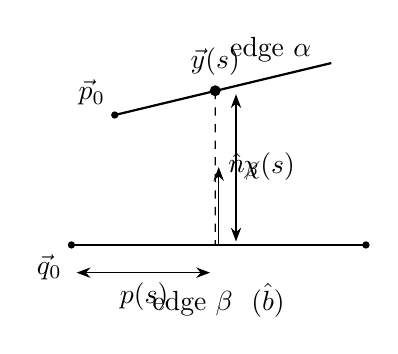
\begin{tikzpicture}[scale=2.2,>={Stealth[length=5pt]}]
  \draw[thick] (0,0) -- (1.7,0);
  \node at (0.85,-0.32) {edge $\beta$ \ ($\hat b$)};
  \fill (0,0) circle (0.6pt) node[below left]{$\vec q_0$};
  \fill (1.7,0) circle (0.6pt);
  \draw[->] (0.85,0) -- (0.85,0.45) node[right]{$\hat n_\beta$};
  \draw[thick] (0.25,0.75) -- (1.5,1.05);
  \node at (1.15,1.13) {edge $\alpha$};
  \fill (0.25,0.75) circle (0.6pt) node[above left]{$\vec p_0$};
  \coordinate (y) at (0.83,0.89);
  \fill (y) circle (0.9pt) node[above=2pt]{$\vec y(s)$};
  \draw[dashed] (y) -- (0.83,0);
  \draw[dashed] (0,0) -- (0.83,0);
  \draw[<->] (0.03,-0.16) -- (0.80,-0.16);
  \node at (0.42,-0.30) {$p(s)$};
  \draw[<->] (0.95,0.02) -- (0.95,0.87);
  \node at (1.14,0.45) {$\chi(s)$};
\end{tikzpicture}
\caption{The edge-pair frame (\S\ref{sec:coords}).  In edge $\beta$'s frame ($\hat b$
along, $\hat n_\beta$ across), a field point $\vec y(s)$ on edge $\alpha$ has along-edge
coordinate $p(s)=P_0+P_1s$ and signed height $\chi(s)=X_0+X_1s$.  The softened
perpendicular distance $\sqrt{\chi^2+\sigma^2}$ and endpoint distance $\sqrt{Q_2}$
carry all the analytic content; $\xi=\chi(s)$ is the working variable.}
\label{fig:frame}
\end{figure}

\subsection{Elementary master primitives}
\label{sec:masters}

Six indefinite integrals, all elementary, carry the load.  Throughout,
$q(s)=a s^2+bs+c$ with $D=4ac-b^2>0$,
$\Theta(\xi)=\atan\!\bigl[(\alpha\xi+\beta)/\sqrt{\xi^2+\sigma^2}\bigr]$, and
$\Delta=\sqrt{\beta^2+(1{+}\alpha^2)\sigma^2}$ (so that $4ac-b^2 = 4\Delta^2$ for
$Q_2$).

\begin{align}
  \Lambda_0(s) &= \int\!\ln q\,\dd s
   = \Bigl(s+\frac{b}{2a}\Bigr)\ln q \;-\;2s\;+\;\frac{\sqrt D}{a}\,
     \atan\frac{2as+b}{\sqrt D},
  \label{eq:Lam0}\\[2pt]
  \Lambda_1(s) &= \int\! s\,\ln q\,\dd s
   = \Bigl(\frac{s^2}{2}-\frac{b^2-2ac}{4a^2}\Bigr)\ln q
     \;-\;\frac{s^2}{2}\;+\;\frac{b\,s}{2a}
     \;-\;\frac{b\sqrt D}{2a^2}\,\atan\frac{2as+b}{\sqrt D},
  \label{eq:Lam1}\\[2pt]
  \Xi_0(\xi) &= \int\!\frac{\dd\xi}{Q_2}
   = \frac{1}{\Delta}\,\atan\frac{(1{+}\alpha^2)\xi+\alpha\beta}{\Delta},
  \qquad
  \Xi_1(\xi) = \int\!\frac{\xi\,\dd\xi}{Q_2}
   = \frac{\ln Q_2}{2(1{+}\alpha^2)}-\frac{\alpha\beta}{1{+}\alpha^2}\,\Xi_0 ,
  \label{eq:Xi}\\[2pt]
  R(\xi) &= \int\!\frac{\xi\,(\alpha\sigma^2-\beta\xi)}{Q_2}\,\dd\xi
   = -\frac{\beta\,\xi}{1{+}\alpha^2}
     +\frac{\alpha\bigl[\sigma^2(1{+}\alpha^2)+2\beta^2\bigr]}{1{+}\alpha^2}\,\Xi_1
     +\frac{\beta\,(\beta^2{+}\sigma^2)}{1{+}\alpha^2}\,\Xi_0 ,
  \label{eq:R}\\[2pt]
  M_1(\xi) &= \int\!\frac{\xi}{\sqrt{\xi^2+\sigma^2}}\,\Theta\,\dd\xi
   = \sqrt{\xi^2+\sigma^2}\;\Theta
     \;+\;\frac{\beta}{2(1{+}\alpha^2)}\,\ln Q_2
     \;-\;\frac{\alpha\Delta}{1{+}\alpha^2}\,
        \atan\frac{(1{+}\alpha^2)\xi+\alpha\beta}{\Delta}.
  \label{eq:M1}
\end{align}
The derivations are one integration by parts each, using the key derivative
\begin{equation}
  \frac{\dd\Theta}{\dd\xi}
  \;=\; \frac{\alpha\sigma^2-\beta\,\xi}{\sqrt{\xi^2+\sigma^2}\;Q_2(\xi)} ,
  \label{eq:dTheta}
\end{equation}
whose numerator is linear and whose denominator is exactly the
perpendicular--endpoint distance pair: integrating $\Theta$ against
$\dd\bigl(\sqrt{\xi^2+\sigma^2}\bigr)=\xi\,\dd\xi/\sqrt{\xi^2+\sigma^2}$ cancels the
square root and leaves a rational integrand --- hence $M_1$ is elementary.
Equation \eqref{eq:M1} was additionally verified by direct differentiation.

\paragraph{The derivations, worked.}  Each master is one integration by parts or one
algebraic reduction; we record them so every coefficient can be reproduced.

\emph{$\Lambda_0=\int\ln q\,\dd s$.}  This is the indefinite log panel: by parts as
above, $\int\ln q\,\dd s = s\ln q-\int s(2as+b)/q\,\dd s$, and the same numerator
substitution $2as^2+bs=2q-(bs+2c)$ with the split
$bs+2c=\tfrac{b}{2a}(2as+b)+\tfrac{D}{2a}$ gives
$\int s(2as+b)/q\,\dd s = 2s-\tfrac{b}{2a}\ln q-\tfrac{D}{2a}\cdot
\tfrac{2}{\sqrt D}\atan\tfrac{2as+b}{\sqrt D}$.  Since
$\tfrac{D}{2a}\cdot\tfrac{2}{\sqrt D}=\tfrac{\sqrt D}{a}$, collecting yields
\eqref{eq:Lam0}.  $\Lambda_1$ is by parts with $v=s^2/2$, followed by one polynomial
division of $s^2(2as+b)$ by $q$ to reduce the integrand to
(constant)$+$(linear)$/q$.

\emph{$\Xi_0,\Xi_1=\int\{1,\xi\}\,\dd\xi/Q_2$.}  Completing the square,
$Q_2=(1{+}\alpha^2)\bigl[(\xi+\tfrac{\alpha\beta}{1+\alpha^2})^2+
\tfrac{\Delta^2}{(1+\alpha^2)^2}\bigr]$, exposes the arctangent \eqref{eq:Xi} with
scale $\Delta$ (this is where $4ac-b^2=4\Delta^2$ for $Q_2$ comes from).  For $\Xi_1$
write $\xi=\tfrac{1}{2(1+\alpha^2)}\bigl[Q_2'(\xi)-2\alpha\beta\bigr]$; the $Q_2'$ part
integrates to $\tfrac{\ln Q_2}{2(1+\alpha^2)}$ and the constant part to
$-\tfrac{\alpha\beta}{1+\alpha^2}\Xi_0$.

\emph{$R=\int\xi(\alpha\sigma^2-\beta\xi)/Q_2\,\dd\xi$.}  Split as
$\alpha\sigma^2\Xi_1-\beta\int\xi^2/Q_2$ and reduce the quadratic numerator with
$\xi^2=\tfrac{1}{1+\alpha^2}\bigl[Q_2-2\alpha\beta\,\xi-(\beta^2{+}\sigma^2)\bigr]$, so
$\int\xi^2/Q_2=\tfrac{1}{1+\alpha^2}\bigl[\xi-2\alpha\beta\,\Xi_1
-(\beta^2{+}\sigma^2)\Xi_0\bigr]$.  Collecting the $\Xi_1$ coefficient
$\alpha\sigma^2+\tfrac{2\alpha\beta^2}{1+\alpha^2}
=\tfrac{\alpha[\sigma^2(1+\alpha^2)+2\beta^2]}{1+\alpha^2}$ gives \eqref{eq:R}.

\emph{$M_1=\int\tfrac{\xi}{\sqrt{\xi^2+\sigma^2}}\,\Theta\,\dd\xi$ --- the one that
matters.}  Integrate by parts against
$\dd\!\sqrt{\xi^2+\sigma^2}=\xi\,\dd\xi/\sqrt{\xi^2+\sigma^2}$:
\[
  M_1 = \sqrt{\xi^2+\sigma^2}\,\Theta
        \;-\;\int \sqrt{\xi^2+\sigma^2}\;\Theta'\,\dd\xi .
\]
The key derivative \eqref{eq:dTheta} carries $\sqrt{\xi^2+\sigma^2}$ in its
denominator, so it \emph{cancels} the arc-length factor and the remainder is
\emph{rational},
$\int(\alpha\sigma^2-\beta\xi)/Q_2\,\dd\xi=\alpha\sigma^2\,\Xi_0-\beta\,\Xi_1$;
substituting $\Xi_1$ and $\Delta^2=\beta^2+(1{+}\alpha^2)\sigma^2$ yields
\eqref{eq:M1}.  This single cancellation --- the softened perpendicular distance in
$\Theta'$ matching the boundary arc-length element --- is the reason the vertex
gradient stays elementary while the energy (which needs one more antiderivative order,
\S\ref{sec:T}) does not.

\subsection{The transcendental core $\mathcal T$}
\label{sec:T}

One further antiderivative order is needed twice: for the energy
($\int\!\sqrt{\xi^2+\sigma^2}\,\Theta\,\dd\xi$) and for the linear-weighted gradient
($\int\!\xi^2(\xi^2+\sigma^2)^{-1/2}\,\Theta\,\dd\xi$).  Both integrate by parts
through
\begin{equation}
  V_\pm(\xi) = \tfrac12\Bigl[\xi\sqrt{\xi^2+\sigma^2}
               \pm \sigma^2\,\asinh(\xi/\sigma)\Bigr],
  \qquad
  V_+'=\sqrt{\xi^2+\sigma^2},\quad V_-'=\frac{\xi^2}{\sqrt{\xi^2+\sigma^2}} ,
\end{equation}
and the $\xi\sqrt{\cdot}$ halves of $V_\pm$ produce the elementary $R$ of
\eqref{eq:R}.  The $\asinh$ halves produce the single transcendental object of the
whole theory,
\begin{equation}
  \mathcal T(\xi) \;=\;
  \int \asinh\!\Bigl(\frac{\xi}{\sigma}\Bigr)\,
  \frac{\alpha\sigma^2-\beta\,\xi}{\sqrt{\xi^2+\sigma^2}\;Q_2(\xi)}\;\dd\xi ,
  \label{eq:Tdef}
\end{equation}
in terms of which
\begin{equation}
  M_2 = \int\!\sqrt{\xi^2{+}\sigma^2}\,\Theta\,\dd\xi
      = V_+\Theta-\tfrac12 R-\tfrac{\sigma^2}{2}\mathcal T ,
  \qquad
  M_1' = \int\!\frac{\xi^2\,\Theta}{\sqrt{\xi^2{+}\sigma^2}}\,\dd\xi
       = V_-\Theta-\tfrac12 R+\tfrac{\sigma^2}{2}\mathcal T .
  \label{eq:M2M1p}
\end{equation}
$\mathcal T$ closes in dilogarithms under the Euler substitution
\begin{equation}
  \eta \;=\; \xi+\sqrt{\xi^2+\sigma^2}\;\in(0,\infty),
  \qquad
  \xi=\frac{\eta^2-\sigma^2}{2\eta},\quad
  \frac{\dd\xi}{\sqrt{\xi^2+\sigma^2}}=\frac{\dd\eta}{\eta},\quad
  \asinh(\xi/\sigma)=\ln(\eta/\sigma) ,
\end{equation}
under which $Q_2=\mathcal Q(\eta)/(4\eta^2)$ with the quartic
\begin{equation}
  \mathcal Q(\eta) = (1{+}\alpha^2)(\eta^2{-}\sigma^2)^2
                     + 4\alpha\beta\,\eta(\eta^2{-}\sigma^2)
                     + 4(\beta^2{+}\sigma^2)\,\eta^2 ,
\end{equation}
and $\alpha\sigma^2-\beta\xi = N(\eta)/2\eta$ with
$N(\eta)=-\beta\eta^2+2\alpha\sigma^2\eta+\beta\sigma^2$.  Hence
$\mathcal T = 2\!\int \ln(\eta/\sigma)\,N(\eta)/\mathcal Q(\eta)\,\dd\eta$; partial
fractions over the four simple roots $\eta_k$ of $\mathcal Q$ and the identity
$\int \ln\eta\,(\eta-a)^{-1}\dd\eta = \ln\eta\,\ln(1-\eta/a)+\Li(\eta/a)$ give
\begin{equation}
  \boxed{\;
  \mathcal T(\xi) \;=\; 2\,\operatorname{Re}\sum_{k=1}^{4}
  \frac{N(\eta_k)}{\mathcal Q'(\eta_k)}
  \Bigl[\ln\!\frac{\eta}{\sigma}\,\ln\!\Bigl(1-\frac{\eta}{\eta_k}\Bigr)
        +\Li\!\Bigl(\frac{\eta}{\eta_k}\Bigr)\Bigr] \;}
  \label{eq:Tclosed}
\end{equation}
with $\mathcal Q'(\eta)=4(1{+}\alpha^2)\eta(\eta^2{-}\sigma^2)
+4\alpha\beta(3\eta^2{-}\sigma^2)+8(\beta^2{+}\sigma^2)\eta$ and the roots obtained
stably from the two conjugate roots of $Q_2$,
\begin{equation}
  \zeta_\pm=\frac{-\alpha\beta\pm i\,\Delta}{1+\alpha^2},
  \qquad
  \eta \in \bigl\{\zeta_\pm \pm \sqrt{\zeta_\pm^2+\sigma^2}\bigr\}
  \quad(\text{four values}).
  \label{eq:roots}
\end{equation}
Each $\zeta$'s two $\eta$-roots multiply to $-\sigma^2$, and the roots come in
conjugate pairs, which is why the real part in \eqref{eq:Tclosed} suffices.

\paragraph{Working the substitution.}  The Euler map straightens both hard factors at
once.  From $\eta=\xi+\sqrt{\xi^2+\sigma^2}$ one has
$\eta-\xi=\sqrt{\xi^2+\sigma^2}$, hence $\eta^2-2\eta\xi=\sigma^2$, giving
$\xi=(\eta^2-\sigma^2)/2\eta$ and $\sqrt{\xi^2+\sigma^2}=(\eta^2+\sigma^2)/2\eta$;
differentiating the first, $\dd\xi/\sqrt{\xi^2+\sigma^2}=\dd\eta/\eta$, and
$\asinh(\xi/\sigma)=\ln(\eta/\sigma)$.  Substituting $\xi$ into $Q_2$ and clearing the
$2\eta$ denominators yields $Q_2=\mathcal Q(\eta)/4\eta^2$ with the quartic
$\mathcal Q$, while the linear numerator becomes $\alpha\sigma^2-\beta\xi=N(\eta)/2\eta$.
The whole integrand then collapses to a logarithm over a quartic:
\[
  \asinh\!\frac{\xi}{\sigma}\,
  \frac{\alpha\sigma^2-\beta\xi}{\sqrt{\xi^2+\sigma^2}\,Q_2}\,\dd\xi
  \;=\; \ln\!\frac{\eta}{\sigma}\cdot
        \frac{N/2\eta}{\mathcal Q/4\eta^2}\cdot\frac{\dd\eta}{\eta}
  \;=\; 2\,\ln\!\frac{\eta}{\sigma}\,\frac{N(\eta)}{\mathcal Q(\eta)}\,\dd\eta .
\]
Partial fractions over the four simple roots,
$N/\mathcal Q=\sum_k \tfrac{N(\eta_k)}{\mathcal Q'(\eta_k)}(\eta-\eta_k)^{-1}$, reduce
$\mathcal T$ to a sum of $\int\ln\eta\,(\eta-\eta_k)^{-1}\dd\eta$ (the $\ln\sigma$ in
$\ln(\eta/\sigma)$ only adds an integration constant, cancelled in the definite
differences $[\,\cdot\,]_{X_0}^{X_0+X_1}$).  The remaining antiderivative is the
dilogarithm identity
\[
  \int\frac{\ln\eta}{\eta-a}\,\dd\eta
  = \ln\eta\,\ln\!\Bigl(1-\frac{\eta}{a}\Bigr)+\Li\!\Bigl(\frac{\eta}{a}\Bigr),
\]
checked by differentiating with $\Li'(x)=-\ln(1-x)/x$: the two $\ln(1-\eta/a)/\eta$
terms cancel, leaving $-\ln\eta/[a(1-\eta/a)]=\ln\eta/(\eta-a)$.  Assembling over the
four roots gives \eqref{eq:Tclosed}.  \emph{Why one dilogarithm and no more:} the
energy stacks two antiderivatives of a logarithm (once in $t$, once in $s$), and each
$\asinh$ half of $V_\pm$ is the second stack --- so $\Li$ enters exactly at the
double-integration level, never higher.

\paragraph{Branch bookkeeping.}
Formula \eqref{eq:Tclosed} with \emph{principal} branches is globally valid for
endpoint differences, with no branch tracking: (i) $\eta>0$ is real and monotonic in
$\xi$; (ii) $Q_2>0$ forces every $\eta_k$ off the real axis, so as $\eta$ sweeps a
real interval, $\eta/\eta_k$ moves along a straight ray through the origin with
non-real direction --- it can never meet the $\Li$ cut $[1,\infty)$; (iii)
$\operatorname{Im}(1-\eta/\eta_k)=-\eta\operatorname{Im}(1/\eta_k)$ has fixed sign,
so the principal $\ln(1-\eta/\eta_k)$ is continuous along the path; and (iv)
integration constants (including the $\ln\sigma$ cross terms) cancel in primitive
differences.  \aside{Verified: $\mathcal T$, $M_2$, $M_1'$ against adaptive
quadrature over random $(\alpha,\beta,\sigma)$ and sign-changing $\xi$-ranges,
agreement at the $10^{-24}$ level at 25-digit precision.}  On dilogarithm identities
(inversion, Landen) useful for range reduction and fast evaluation see
\cite{Lewin1981,DLMF}.

\paragraph{Evaluating the dilogarithm.}  In practice $\Li(z)$ on complex $z$ is computed
by range reduction to $|z|\le\tfrac12$, where the series $\Li(z)=\sum_{k\ge1}z^k/k^2$
converges quickly, using the inversion
$\Li(z)+\Li(1/z)=-\tfrac{\pi^2}{6}-\tfrac12\ln^2(-z)$ for $|z|>1$ and the reflection
$\Li(z)+\Li(1-z)=\tfrac{\pi^2}{6}-\ln z\,\ln(1-z)$ (or the Landen map
$\Li(z)=-\Li(\tfrac{z}{z-1})-\tfrac12\ln^2(1-z)$) to pull the argument into that disk
\cite{Lewin1981,DLMF}.  \aside{The oracle uses \texttt{mpmath.polylog}; the numpy port
uses \texttt{scipy.special.spence}, related by $\Li(z)=\mathrm{spence}(1-z)$ and matched
to $\sim10^{-16}$ against \texttt{mpmath} on real and complex arguments; a GPU kernel
would inline the reduced series.}  Because the four roots per pair share $\zeta_\pm$, an
implementation computes them once and calls $\Li$ four times (energy) or eight (energy
$+$ gradient) per non-parallel edge pair.

\subsection{Assembled energy}
\label{sec:energyassembled}

The pair integral $I_{\alpha\beta}=\int_0^1\!\int_0^1\ln Q\,\dd s\,\dd t$ evaluates
by doing $t$ first with the log panel (in the $u$-variable,
$\int\!\ln(u^2+h^2)\,\dd u = u\ln(u^2+h^2)-2u+2h\atan(u/h)$) and then $s$ with the
masters:
\begin{equation}
  \boxed{\;
  I_{\alpha\beta} \;=\; \frac{1}{L_B}\sum_{e\in\{0,1\}} \epsilon_e\,
  \Bigl[\,\mathcal A_e \;-\; 2\,\mathcal B_e \;+\; 2\,\mathcal C_e\,\Bigr]\;}
  \label{eq:Iassembled}
\end{equation}
with, per endpoint $e$ (all bracketed primitives evaluated between the stated
limits),
\begin{align}
  \mathcal A_e &= \int_0^1 u_e\,\ln q_e\,\dd s
   \;=\; U_{0e}\,\bigl[\Lambda_0\bigr]_0^1+P_1\,\bigl[\Lambda_1\bigr]_0^1
   \qquad\text{on } q_e \text{ of \eqref{eq:qe}},
  \\
  \mathcal B_e &= \int_0^1 u_e\,\dd s \;=\; U_{0e}+\tfrac12 P_1 ,
  \\
  \mathcal C_e &= \int_0^1 h\,\atan\frac{u_e}{h}\,\dd s
   \;=\;
   \begin{cases}
     \dfrac{1}{X_1}\Bigl[M_2\bigl(\xi;\alpha,\beta_e\bigr)\Bigr]_{X_0}^{X_0+X_1}
       & X_1\neq0,\\[8pt]
     \dfrac{h}{P_1}\Bigl[u\,\atan\dfrac{u}{h}-\dfrac{h}{2}\ln(u^2{+}h^2)
       \Bigr]_{U_{0e}}^{U_{0e}+P_1},\quad h=\sqrt{X_0^2+\sigma^2}
       & X_1=0 ,
   \end{cases}
  \label{eq:Ce}
\end{align}

\paragraph{How the pieces arise.}  Do the inner ($t$) integral first.  In the
variable $u=p(s)-L_B t$ (so $Q=u^2+h^2$ and $\dd t=-\dd u/L_B$), the log panel is
$\int\ln(u^2+h^2)\dd u=u\ln(u^2+h^2)-2u+2h\atan(u/h)$, evaluated between the two
$B$-endpoints $u_0(s)=p(s)$ and $u_1(s)=p(s)-L_B$.  Written as a signed sum over
$e\in\{0,1\}$ ($\epsilon_0{=}{+}1$, $\epsilon_1{=}{-}1$) and divided by the Jacobian
$L_B$, it leaves three outer $s$-integrals per endpoint.  The $u\ln(u^2+h^2)$ term is
$\mathcal A_e=\int_0^1 u_e\ln q_e\,\dd s$ --- done by $\Lambda_0,\Lambda_1$, since
$u_e=U_{0e}+P_1s$ is linear and $q_e$ is the quadratic \eqref{eq:qe}; the $-2u$ term is
$-2\mathcal B_e$ with $\mathcal B_e=\int_0^1 u_e\,\dd s$, trivial; and the
$2h\atan(u/h)$ term is $2\mathcal C_e$ --- the \emph{only} place $\Theta$ (hence $M_2$,
hence $\mathcal T$) enters.  So the endpoint sum \eqref{eq:Iassembled} is just the two
evaluation limits of the inner log panel, propagated through the outer integral.

\noindent and the total mollified overlap
\begin{equation}
  \Acap \;=\; -\frac{1}{4\pi}\sum_{\alpha\in\partial A}\sum_{\beta\in\partial B}
  (\hat n_\alpha\!\cdot\!\hat n_\beta)\,L_A L_B\; I_{\alpha\beta}\, .
  \label{eq:Atotal}
\end{equation}
Parallel edges ($X_1=0$, in which case $P_1=\pm L_A\neq0$) are \emph{fully
elementary}; the non-parallel case costs, per endpoint, one evaluation of
\eqref{eq:Tclosed}, i.e.\ four complex dilogarithms and logarithms at each of the two
$\xi$-limits.  \aside{Verified: \eqref{eq:Iassembled} against tensor quadrature of
$\ln Q$ over random edge pairs (crossing, disjoint, exactly parallel) to
$\sim10^{-24}$; the full double sum \eqref{eq:Atotal} against area quadrature of
$\int_A\Psi_B$ for two overlapping quadrilaterals to $4\times10^{-25}$.}

\subsection{Assembled gradient}
\label{sec:gradassembled}

The vertex forces \eqref{eq:vertexforce} need the hat-weighted moments of
$\Psi_B$ along each $A$-edge.  Per $B$-edge $\beta$, writing \eqref{eq:psiedge} in
pair coordinates ($\vec w\cdot\hat n_\beta = -\chi$, $w_\parallel=-p$),
\begin{equation}
  \psi_\beta(s) \;=\; -\frac{\chi(s)}{2\pi\,h(s)}
  \sum_{e}\epsilon_e\,\atan\frac{u_e(s)}{h(s)},
  \label{eq:psipair}
\end{equation}
so the required moments $W_m=\int_0^1 s^m\,\psi_\beta\,\dd s$ ($m=0,1$) are, for
$X_1\neq0$,
\begin{equation}
  \boxed{\;
  \begin{aligned}
  W_0 &= -\frac{1}{2\pi X_1}\sum_e \epsilon_e
        \Bigl[M_1(\xi;\alpha,\beta_e)\Bigr]_{X_0}^{X_0+X_1},\\
  W_1 &= -\frac{1}{2\pi X_1^2}\sum_e \epsilon_e
        \Bigl[M_1'(\xi;\alpha,\beta_e)-X_0\,M_1(\xi;\alpha,\beta_e)
        \Bigr]_{X_0}^{X_0+X_1}
  \end{aligned}\;}
  \label{eq:Wclosed}
\end{equation}

\paragraph{Deriving the moments.}  Substitute $\xi=\chi(s)=X_0+X_1s$ in
\eqref{eq:psipair}: $s=(\xi-X_0)/X_1$, $\dd s=\dd\xi/X_1$, and with $\chi=\xi$,
$h=\sqrt{\xi^2+\sigma^2}$ the integrand becomes (up to $-1/2\pi$)
$s^m\,\tfrac{\xi}{\sqrt{\xi^2+\sigma^2}}\sum_e\epsilon_e\,\Theta(\xi;\alpha,\beta_e)$.
For $m=0$ this is $\tfrac{\xi}{\sqrt{\cdot}}\Theta$, whose antiderivative is $M_1$ ---
giving $W_0$.  For $m=1$, splitting $s=(\xi-X_0)/X_1$ produces
$\tfrac{\xi^2}{\sqrt{\cdot}}\Theta$ and $-X_0\tfrac{\xi}{\sqrt{\cdot}}\Theta$, with
antiderivatives $M_1'$ and $-X_0M_1$ --- giving $W_1$; the extra powers of $1/X_1$ are
the substitution Jacobians.  Since $M_1$ is elementary and only $M_1'$ carries
$\mathcal T$, the net edge force $W_0$ is elementary and the dilogarithm sits solely in
the linear apportionment $W_1$, as noted next.

The parallel case is again elementary, using the arctangent primitive of
\eqref{eq:Ce} together with
\begin{equation*}
  \int\! u\,\atan\frac{u}{h}\,\dd u
  \;=\; \frac{u^2{+}h^2}{2}\,\atan\frac{u}{h}\;-\;\frac{h\,u}{2}\, .
\end{equation*}
The force deposit on the edge from $\vec v_m$ to $\vec v_{m+1}$ is
\begin{equation}
  \frac{\partial\Acap}{\partial\vec v_m}\;{+}{=}\;
  L_A\,\nA \sum_{\beta\in\partial B}\bigl(W_0-W_1\bigr),
  \qquad
  \frac{\partial\Acap}{\partial\vec v_{m+1}}\;{+}{=}\;
  L_A\,\nA \sum_{\beta\in\partial B} W_1 ,
  \label{eq:deposit}
\end{equation}
plus the mirror-image contributions on $\partial B$ with $\Psi_A$.  Two structural
remarks.  First, $W_0$ --- the \emph{net} force integral of an edge --- is purely
elementary: dilogarithms enter only through the linear apportionment $W_1$, i.e.\
exactly at the piecewise-linear (Galerkin) level, in agreement with the symmetric
Galerkin analytic-integration literature \cite{Carini1999,Salvadori2002}.  Second,
$W_0,W_1$ reuse the same $(\alpha,\beta_e)$ and root data as the energy, so an
implementation computes $\zeta_\pm,\eta_k$ once per edge pair.  \aside{Verified:
\eqref{eq:Wclosed} against quadrature of $s^m\psi_\beta$ to $\sim10^{-23}$, and the
fully assembled $\partial\Acap/\partial\vec v$ (all vertices, both polygons) against
central finite differences of the closed-form energy to $1\times10^{-13}$ ---
FD-limited.}

\subsection{Worked case: parallel edges}
\label{sec:parallel}

The parallel branch ($X_1=0$) is worth carrying through in full: it is the elementary
skeleton, and near-aligned edges are generic at jamming, so a production code runs it
often.  Here $\chi(s)\equiv X_0$ is a fixed signed gap, $h=\sqrt{X_0^2+\sigma^2}$ is
constant, and $P_1=\pm L_A$; take $P_1=L_A$ (co-oriented edges).  The endpoint abscissa
is $u_e(s)=U_{0e}+L_As$ with $U_{0e}=P_0-eL_B$, and $q_e=u_e^2+h^2$.  Changing to
$u=u_e$ ($\dd s=\dd u/L_A$), each master collapses to a standard endpoint evaluation:
\[
  \mathcal A_e=\frac{1}{L_A}\Bigl[\tfrac12(u^2{+}h^2)\ln(u^2{+}h^2)-\tfrac12 u^2
     \Bigr]_{U_{0e}}^{U_{0e}+L_A},\quad
  \mathcal B_e=U_{0e}+\tfrac12 L_A,\quad
  \mathcal C_e=\frac{h}{L_A}\Bigl[u\,\atan\tfrac{u}{h}-\tfrac{h}{2}\ln(u^2{+}h^2)
     \Bigr]_{U_{0e}}^{U_{0e}+L_A},
\]
using $\int u\ln(u^2{+}h^2)\dd u=\tfrac12(u^2{+}h^2)\ln(u^2{+}h^2)-\tfrac12 u^2$ (mod a
constant that cancels in the difference) and the arctangent primitive of
\eqref{eq:Ce}.  There is no $\mathcal T$, no dilogarithm, no complex arithmetic: the
whole edge-pair energy
$I_{\alpha\beta}=L_B^{-1}\sum_e\epsilon_e[\mathcal A_e-2\mathcal B_e+2\mathcal C_e]$
is four logarithms and four arctangents of the corner distances and angles, exactly
the $\sigma$-softened version of the sharp parallel-strip overlap.  Geometrically it
depends only on the perpendicular gap (through $h$) and on how far the two edges
overlap when projected onto their common direction (through the $U_{0e}$); as
$\sigma\to0$, $h\to|X_0|$ and it reduces to the elementary area of the overlapping
parallel strip.  This is the branch the near-parallel limit (\S\ref{sec:cost}) is
matched to.

\subsection{Consistency checks the closed forms satisfy}
\label{sec:checks}

Four invariances double as correctness checks on an implementation.
\emph{Translation invariance:} rigidly translating a polygon leaves every pairwise
overlap unchanged, so the net overlap force on it vanishes,
$\sum_m\partial\Acap/\partial\vec v_m=\vec0$ --- the two hat deposits \eqref{eq:deposit}
must cancel across a polygon; verified to $\sim10^{-15}$.  \emph{Newton's third law:}
since \eqref{eq:energy} is symmetric in $A\leftrightarrow B$, the force a translation of
$A$ feels from $B$ is minus that $B$ feels from $A$, so momentum is conserved pairwise.
\emph{Gauge:} adding a constant to $\Phi$ changes nothing, by
$\oint\hat n\,\dd\ell=\vec0$, so only \emph{differences} of the softened log across a
pair contribute --- the origin of the far-pair cancellation (\S\ref{sec:cost}).
\emph{Sharp limit:} $\sigma\to0$ collapses every formula onto the elementary
complex-corner skeleton \S\ref{sec:sharp}, the explicit $\sigma^2$ prefactors on the
$\mathcal T$ sector switching the dilogarithms off (\S\ref{sec:sharplimit}).  The first
two are the cheapest live guards against a sign or index slip, and a production code
should assert them at every step.

\subsection{Degenerate limits, conditioning, and cost}
\label{sec:cost}

\emph{Near-parallel edges.}  As $X_1\to0$, $\alpha=\cot\theta\to\infty$ and
\eqref{eq:Wclosed}--\eqref{eq:Ce} become a difference of large quantities.  The
formulas remain exact; a float64 production code should nevertheless switch to the
elementary parallel branch below a threshold $|X_1|\lesssim\varepsilon L_A$ and, if
needed, bridge with a
first-order expansion in $X_1$ --- the standard panel-method treatment
\cite{KatzPlotkin2001}.  The instability is superficial: each moment is a difference
quotient in the limits $X_0$ and $X_0+X_1$ (e.g.\ $\mathcal C_e,W_0\sim
[F]_{X_0}^{X_0+X_1}/X_1$), exact for all $X_1$ but cancellation-prone as $X_1\to0$; its
limit is the derivative $F'(X_0)$, which \emph{is} the parallel-branch formula (a segment
at fixed height $X_0$).  So the two branches meet smoothly, and a first-order Taylor
expansion of the difference quotients removes the cancellation analytically if a single
code path is wanted.  \emph{Far pairs.}  By $\oint\hat n\,\dd\ell=0$ the constant
part of the log cancels between edges, so distant pairs are computed as small
differences of $\mathcal O(\ln r)$ terms; evaluating pairs in a local frame centered
on the pair and compensated summation keep this benign; beyond the switch radius
(\S\ref{sec:switch}) far pairs are absent altogether.  \emph{Root degeneracies.}
The $\eta_k$ are simple and nonzero for all $\sigma>0$ except at isolated parameter
points ($\alpha=\beta=0$, where $\Theta\equiv0$ and $\mathcal T$ is not needed); a
guard suffices.

\emph{Operation count.}  Per non-parallel edge pair, the energy costs
$2\times$\eqref{eq:Tclosed} $=8$ complex dilogarithms $+\,8$ complex logs, plus
$\mathcal O(10)$ real $\ln/\atan/\sqrt{\cdot}/\asinh$; the gradient adds the same
$\mathcal T$ data plus a handful of elementary terms.  The semi-analytic tier at
$G=32$ spends roughly $32\times$ a few real transcendentals per pair, so the closed
form is an order of magnitude fewer transcendental evaluations --- \aside{consistent
with the observed 11$\times$ from removing the previous quadrature level} --- with
the caveat that complex arithmetic and $\Li$ evaluations (series plus
inversion/Landen reductions \cite{Lewin1981}; \texttt{mpmath}/\texttt{scipy} host
side) are individually more expensive than a real $\atan$.  The qualitative win is
accuracy: machine-exact independent of $\sigma$ and of how the boundaries cross, so
$\sigma$ can be pushed down without raising any quadrature order.
\aside{Status: the fully analytic tier is derived and verified end-to-end in
\texttt{verify\_plummer\_analytic.py} (this document's companion); the CUDA port in
\texttt{pyCudaPolygon} is pending, with the complex-$\Li$ kernel the only new
device primitive.}

%======================================================================
\section{Tail, truncation, and kernel selection}
\label{sec:tail}
%======================================================================

Three error mechanisms separate $\Acap$ from the true overlap.  (i)~\emph{Far-pair
tail}: for disjoint bodies at separation $r\gg\sigma$, expanding \eqref{eq:defA}
gives $\Acap\approx A_A A_B\,K_\sigma(r)=\sigma^2 A_A A_B/(\pi r^4)$ --- spurious but
smooth, vanishing as $\sigma^2$; it is the price of forbidding cutoffs.
(ii)~\emph{Straight-boundary crossings}: where $\partial B$ passes through the
interior of $A$, the soft step \eqref{eq:step} is odd about $\tfrac12$, so the
leading-order error integrates to zero along straight portions; net contributions
arise only within $\mathcal O(\sigma)$ of $\partial A\cap\partial B$ intersection
points, each contributing $\mathcal O(\sigma^2)$.  (iii)~\emph{Corners}: each corner
of one polygon inside the other contributes $\mathcal O(\sigma^2)$ with an
angle-dependent coefficient.  A caution on sharpening these statements: the Plummer
kernel's radial second moment $\int r^2K_\sigma\,\dd^2r$ diverges logarithmically, so
the usual moment-condition bookkeeping of blob kernels \cite{BealeMajda1985} does not
apply verbatim, and logarithmic corrections to the $\sigma^2$ scalings should not
surprise.  \aside{Empirically the pair energy converges to the exact overlap as
$\sigma\to0$ (checked in \texttt{plummerPairEnergy}); a measured convergence-order
plot is still to be produced.}

\subsection{How bad is the tail, quantitatively?}
\label{sec:tailsize}

Normalize the rational family as
$K^{(m)}_\sigma=(m/\pi)\,\sigma^{2m}/(r^2+\sigma^2)^{m+1}$, so $m{=}1$ is
\eqref{eq:kernel}.  For two disjoint bodies at center separation $r$ large compared
with their sizes,
\begin{equation}
  E_{\text{tail}}(r)\simeq\frac{m}{\pi}\,\frac{\sigma^{2m}A_AA_B}{r^{2m+2}},
  \qquad
  F_{\text{tail}}(r)\simeq\frac{(2m{+}2)\,m}{\pi}\,
  \frac{\sigma^{2m}A_AA_B}{r^{2m+3}},
  \label{eq:tailforce}
\end{equation}
These follow by factorization: at center separation $r$ much larger than either body
the kernel is nearly constant across each, so \eqref{eq:defA} gives
$\Acap\approx A_AA_B\,K^{(m)}_\sigma(r)$, and
$K^{(m)}_\sigma(r)\approx(m/\pi)\sigma^{2m}r^{-2m-2}$ for $r\gg\sigma$ is
$E_{\text{tail}}$; the force $-\dd E_{\text{tail}}/\dd r$ pulls down the extra
$(2m{+}2)/r$.  So matching the \emph{untruncated} model to a force tolerance
$\varepsilon$ costs a cutoff radius
\begin{equation}
  r_c(\varepsilon)=\Bigl[\frac{(2m{+}2)\,m\,\sigma^{2m}A_AA_B}{\pi\,\varepsilon}
  \Bigr]^{1/(2m+3)}\;\sim\;\varepsilon^{-1/(2m+3)} .
  \label{eq:rc}
\end{equation}
For Plummer ($m{=}1$) at $\sigma=0.05$, $A_A\!\sim\!A_B\!\sim\!1$,
$\varepsilon=10^{-12}$: $r_c\approx80$ --- no useful cutoff exists; the $m{=}3$
member's $\sigma^6/r^8$ tail brings $r_c\approx4$.  The $\varepsilon^{-1/5}$ scaling
is the quantitative content of ``the tail is bad''.  It is also the wrong
requirement, as follows.

\subsection{Smooth truncation}
\label{sec:switch}

``No cutoff'' forbids only \emph{discontinuous} truncation.  Multiply each edge-pair
energy by a smooth switch of the midpoint separation
$r_{\alpha\beta}=|\vec m_\alpha-\vec m_\beta|$,
\begin{equation}
  E_{\alpha\beta}\;\longmapsto\;S(r_{\alpha\beta})\,E_{\alpha\beta},
  \qquad
  S\equiv1 \text{ for } r\le R^{\alpha\beta}_{\text{on}},\quad
  S\equiv0 \text{ for } r\ge R^{\alpha\beta}_{\text{off}},
  \label{eq:switch}
\end{equation}
with $R^{\alpha\beta}_{\text{on/off}}=\tfrac12(L_\alpha{+}L_\beta)+g_{\text{on/off}}$
and a $C^\infty$ bridge between (a standard bump partition; a $C^2$ quintic
smoothstep suffices for FIRE/CG if a transcendental-free switch is preferred).  The
switched model is exactly as smooth as the unswitched one, keeps
force$\,=\nabla$energy \emph{exactly} --- the product-rule term deposits
$\pm\tfrac12 S'E_{\alpha\beta}\,\hat r$ on the four endpoints, since
$\partial\vec m/\partial\vec v=\tfrac12$ --- and, with $g_{\text{on}}$ a few
$\sigma$ beyond genuine contact range, differs from untruncated Plummer only where
the interaction is pure spurious tail: a modification of the same
$\mathcal O(\sigma^{2m})$ size as the mollification bias above, vanishing in the
sharp limit exactly as the bias does.  The switch is therefore part of the model
definition, not an approximation to be $\varepsilon$-matched; \eqref{eq:rc} prices
the stricter requirement one is declining.  Its operational payoff:
$S\equiv0$ beyond $R_{\text{off}}$ makes far edge pairs \emph{identically} zero,
licensing exact gates and reusable neighbor lists (\S\ref{sec:neighbors}).
\aside{Recommended first move: no kernel change, no new analytics --- the closed
forms of \S\ref{sec:outer} are untouched; the switch multiplies them.}

\subsection{Kernel selection}
\label{sec:kernels}

Within full-support radial kernels, nothing cleaner than the softened log exists.
Writing $\vec F=g(u)\,\vec r$ with $u=|\vec r|^2$ gives $K=2\,\dd(ug)/\dd u$, so
normalization forces $ug\to1/2\pi$ at large $u$ and regularity forces $ug\to0$ at
$u=0$; the minimal rational interpolant with a single scale is
$ug=u/[2\pi(u+\sigma^2)]$ --- which \emph{is} Plummer, with
$\Phi=\tfrac12\int g\,\dd u=\ln(u+\sigma^2)/4\pi$.  The logarithm, and with it the
dilogarithm core $\mathcal T$, is structural: every normalized member of the family
carries the same $\ln$ coefficient $1/4\pi$, plus rational corrections.

The derivation template is not tied to \eqref{eq:kernel}.  Any radial rational
kernel, e.g.\ the higher-order family
$K^{(m)}_\sigma\propto\sigma^{2m}/(r^2+\sigma^2)^{m+1}$ with $m\ge2$, has finite
second moment and a faster tail $\sim r^{-2(m+1)}$, permitting neighbor lists in
practice while retaining $C^\infty$.  The radial ODE gives $\vec F$ rational and
$\Phi$ equal to the same softened log plus a rational correction, so the panel
algebra of \S\S\ref{sec:inner}--\ref{sec:outer} carries over with additional
\emph{elementary} terms only ($\mathcal T$ is unchanged in kind).  \aside{This is
the concrete route for the \texttt{TODO.md} item ``faster-decaying rational kernel +
neighbor list for large $N$''.}

Two neighbors outside the rational family are worth recording.  The
Cauchy--Poisson kernel $K=(\sigma/2\pi)(r^2+\sigma^2)^{-3/2}$ has arguably the
prettiest potential and step,
\begin{equation}
  \Phi=\frac{1}{2\pi}\ln\!\bigl(\sigma+\sqrt{r^2+\sigma^2}\,\bigr),
  \qquad
  s(d)=\frac12+\frac1\pi\,\atan\frac d\sigma ,
  \label{eq:cauchy}
\end{equation}
but a slower $\sigma/r^3$ tail, and because $\Phi$ mixes $r$ through
$\sqrt{r^2+\sigma^2}$ its double-panel integrals are no simpler.  The genuinely
different option is a \emph{compactly supported} polynomial kernel
$K_p\propto(1-r^2/\sigma^2)_+^{\,p}$ (Wendland type \cite{Wendland1995}).  By the
two-dimensional shell theorem, $\Phi=\tfrac1{2\pi}\ln r+\text{const}$ \emph{exactly}
for $r\ge\sigma$ (the constant immaterial by $\oint\hat n\,\dd\ell=0$) and an even
polynomial of degree $2p{+}2$ inside; $\Psi_B$ is identically $0$ or $1$ outside a
$\sigma$-collar of $\partial B$, and the pair energy \emph{vanishes identically}
for gaps $>\sigma$: exact neighbor lists with no switch, no tail, no image
subtleties.  Edge pairs with clearance $>\sigma$ use the sharp complex-corner
formula \eqref{eq:sharpcorners} verbatim; near pairs reduce to polynomial double
integrals over the clipped region $Q\le\sigma^2$ (an ellipse--unit-square
intersection) plus the corner formula on the remainder --- elementary throughout, no
$\Li$, but piecewise, and only finitely smooth: $K_p\in C^{p-1}$ at the support edge
gives an energy of class $\approx C^{p+1}$ across branch boundaries, ample for
FIRE/CG at $p=3$--$4$.  Trade summary: Plummer $=$ uniform branch-free formulas, one
transcendental, algebraic tail managed by the switch; compact polynomial $=$ fully
elementary with the best possible complexity, at the price of clipping case
analysis and finite smoothness.  \aside{Default remains Plummer $+$ switch; revisit
the compact kernel if complex $\Li$ proves awkward on the GPU.}

%======================================================================
\section{The sharp limit $\sigma\to0$}
\label{sec:sharplimit}
%======================================================================

By construction the model degenerates to the sharp one: $K_\sigma\to\delta^2$, the
soft step \eqref{eq:step} $\to$ the Heaviside step, $\Psi_B\to$ the winding number
(each edge's arctangent pair in \eqref{eq:psiedge} becomes the true subtended
angle), and $\Acap\to A_\cap$ with the $\mathcal O(\sigma^2)$-up-to-logs bias of
\S\ref{sec:tail}.  The limit is also visible \emph{inside} the closed forms, and
constitutes a nontrivial consistency check: every transcendental piece carries an
explicit $\sigma^2$ prefactor --- the $\asinh$ halves of $V_\pm$ and the entire
$\mathcal T$ sector enter as $\tfrac{\sigma^2}{2}\mathcal T$ in \eqref{eq:M2M1p} ---
while $\mathcal T$ grows at most like $\ln^2(1/\sigma)$, so the dilogarithm content
of the theory switches off as $\sigma^2\ln^2(1/\sigma)$ and the surviving elementary
terms must (and do) reassemble into the sharp complex-corner formula
\eqref{eq:sharpcorners}.  The dilogarithms are genuinely finite-$\sigma$ objects.

\paragraph{The switch-off, in detail.}  In \eqref{eq:M2M1p} the entire dilogarithm
sector enters only as $\pm\tfrac{\sigma^2}{2}\mathcal T$.  As $\sigma\to0$, $\mathcal T$
grows at most like $\ln^2(1/\sigma)$ --- its dilogarithm arguments stay bounded except
near the small roots $\eta\approx-\sigma^2/2\zeta_\pm$ of \eqref{eq:roots}, which supply
the $\ln^2$ --- so $\tfrac{\sigma^2}{2}\mathcal T=\mathcal O(\sigma^2\ln^2(1/\sigma))
\to0$.  The surviving $V_\pm\Theta-\tfrac12 R$ are elementary, and $\Theta$ becomes the
true sharp corner angle $\atan[(\alpha\xi+\beta)/|\xi|]$; they must and do reassemble
into the complex-corner formula \eqref{eq:sharpcorners}.  This reassembly is a
nontrivial check that the integration constants and branch choices of \S\ref{sec:T} are
correct.  Physically, the softening is a finite-$\sigma$ deformation of a genuinely
elementary $\sigma=0$ answer: the dilogarithm is the price of a finite contact width,
not of the geometry.

The convergence is deliberately not uniform in derivatives.  The pair-force
crossover at a contact compresses into a window of width $\sigma$, so landscape
curvature grows as $1/\sigma$ and the stable explicit-integrator step (FIRE is
velocity--Verlet based \cite{Bitzek2006}) shrinks as $\sqrt\sigma$; at small enough
$\sigma$ one has faithfully recovered the sharp model \emph{including} the
hard-stall pathology the mollification exists to escape.  Nor should the formulas
be evaluated \emph{at} $\sigma=0$: self- and collinear panels lose $D>0$ in
\eqref{eq:abcD}, crossing pairs reacquire the logarithmic singularity, and the
small roots $\eta\approx-\sigma^2/2\zeta_\pm$ of \eqref{eq:roots} drive $\Li$
arguments to size $\sigma^{-2}$, requiring the inversion identity \cite{Lewin1981}
and care in float64 --- conditioning degrades before the mathematics does.

Since the analytic tier's cost is $\sigma$-independent (\S\ref{sec:cost}), the
natural protocol is $\sigma$-continuation: relax at generous $\sigma$, anneal
downward, and stop when the $\mathcal O(\sigma^2)$ bias meets the force or
observable tolerance, rather than at the limit itself.  \aside{Not yet scripted;
the $N=6$ endpoint of \S\ref{sec:selfrep} used fixed $\sigma=0.05$.}

%======================================================================
\section{Self-repulsion (self-avoidance)}
\label{sec:selfrep}
%======================================================================

The mollified minimum is meaningful only on \emph{simple} loops: a self-intersecting
polygon has winding $\notin\{0,1\}$, the reduction \eqref{eq:energy} then computes a
winding-weighted area, and folding a flap spuriously lowers the energy --- both FIRE
\cite{Bitzek2006} and CG dive into it if allowed.  \texttt{selfRepulsion.py} adds a
smooth barrier between every non-adjacent edge pair of a polygon,
\begin{equation}
  U_{\text{self}} \;=\; \frac{k_{\text{self}}}{2}\sum_{\text{polygons}}
  \sum_{\text{non-adj }(i,j)} \int_0^1\!\!\int_0^1
  \exp\!\Bigl[-\frac{|\vec y(s)-\vec z(t)|^2}{2\delta^2}\Bigr]\dd s\,\dd t ,
  \label{eq:Uself}
\end{equation}
which is $\approx0$ when non-adjacent edges are $\gtrsim\delta$ apart and rises to
$\sim k_{\text{self}}$ as they approach, blocking the crossing.  \aside{Gaussian
bump, quadratured (few edge pairs per polygon, cheap); FD force $=-\nabla U$ to
$6\times10^{-11}$.  First cut --- form, $k_{\text{self}}$, $\delta$ still to be
pinned.}  Conceptually this is the polygonal cousin of self-avoidance energies for
curves \cite{GonzalezMaddocks1999,YuSchumacherCrane2021}.

The Plummer machinery closes this integral too, and --- pleasantly --- without
dilogarithms.  Replacing the Gaussian bump by the matched rational bump
$\delta^4/Q^2$ with $Q=|\vec y-\vec z|^2+\delta^2$ (maximum $1$ at contact, tail
$\delta^4/r^4$), the required double integral is
\begin{equation}
  S \;=\; \int_0^1\!\!\int_0^1 \frac{\dd s\,\dd t}{Q(s,t)^2}
  \;=\; \frac{1}{2L_B X_1}\sum_e \epsilon_e \int_{X_0}^{X_0+X_1}
        \Bigl[\frac{\alpha\xi+\beta_e}{(\xi^2{+}\delta^2)\,Q_2}
        +\frac{\Theta_e}{(\xi^2{+}\delta^2)^{3/2}}\Bigr]\dd\xi ,
  \label{eq:S}
\end{equation}
(inner $t$-integral by the standard $\int\!\dd t/q^2$ reduction; $\sigma\to\delta$
throughout in $Q_2$, $\Theta$, $\zeta_\pm$), where the first
term is rational --- residues over the four poles $\{\pm i\delta,\zeta_\pm\}$, summed
as $\operatorname{Re}\sum_k r_k\ln(\xi-\xi_k)$ --- and the second closes by parts,
\begin{equation}
  \int\!\frac{\Theta\,\dd\xi}{(\xi^2{+}\delta^2)^{3/2}}
  \;=\; \frac{\xi\,\Theta}{\delta^2\sqrt{\xi^2+\delta^2}}
  \;-\;\frac{1}{\delta^2}\int\!\frac{\xi(\alpha\delta^2-\beta\xi)}
       {(\xi^2{+}\delta^2)\,Q_2}\,\dd\xi ,
  \label{eq:Mm3}
\end{equation}
whose remainder is again rational: \emph{fully elementary}, parallel case included;
retaining the prefactor convention of \eqref{eq:Uself}, each non-adjacent pair
contributes $\tfrac{k_{\text{self}}}{2}\,\delta^4 S$.
The vertex gradient follows by differentiating the closed form with respect to the
four endpoints (mechanical; no new transcendentals).  \aside{Equation \eqref{eq:S}
verified against tensor quadrature to $3\times10^{-22}$.  Swapping
\eqref{eq:Uself}'s Gaussian for the rational bump would make the barrier
quadrature-free and $C^\infty$ with an algebraic tail --- consistent with the
overlap kernel --- at the cost of the same no-cutoff constraint; whether the
$\delta^4/r^4$ tail between distant edges of a large floppy polygon matters is a
question for the $k_{\text{self}},\delta$ pinning pass.}

\paragraph{The inner reduction, worked.}  The barrier's inner integral is the standard
$\int_0^1\dd t/Q^2$.  In $u=p(s)-L_Bt$ (so $Q=u^2+h^2$),
\[
  \int\frac{\dd u}{(u^2+h^2)^2}
  = \frac{u}{2h^2(u^2+h^2)}+\frac{1}{2h^3}\atan\frac uh ,
\]
so evaluating between the two $B$-endpoints and passing to $\xi=\chi(s)$
($h^2=\xi^2+\delta^2$, $u^2+h^2=Q_2$) yields exactly the two $s$-integrands of
\eqref{eq:S}: a rational one, and $\Theta/(\xi^2+\delta^2)^{3/2}$.  The rational
$s$-integral is a sum of residues over the four poles $\{\pm i\delta,\zeta_\pm\}$ ---
the softened-perpendicular pair $\pm i\delta$ and the endpoint pair $\zeta_\pm$ --- and
the second closes by parts \eqref{eq:Mm3} into another rational integral.  No
$\Theta$-primitive of the $M_2/\mathcal T$ kind is needed, so the barrier is
dilogarithm-free even though it reuses the same $Q_2,\zeta_\pm$ data as the overlap:
the extra power in $Q^2$ (versus $\ln Q$) trades the transcendental for a
higher-order rational.

\paragraph{End-to-end status.}
\aside{FIRE on $\Acap+U_{\text{eqSoftBody}}+U_{\text{self}}$ ($N=6$,
$\sigma=\delta=0.05$, $k=1$) relaxes to $\max|F|=9.9\times10^{-9}$ in 2159 steps
($\sim3$\,min), simple throughout --- the machine-precision, fold-free minimization
the sharp model cannot reach (its gradient jumps at contact; sharp CG from this
minimum hard-stalls at $\max|F|\approx3.6\times10^{-3}$).}

%======================================================================
\section{Neighbor lists, images, and global complexity}
\label{sec:neighbors}
%======================================================================

With the switch of \S\ref{sec:switch} (or a compact kernel, \S\ref{sec:kernels})
far pairs are identically zero, and the current all-pairs-times-$3{\times}3$-images
sum --- $\Theta(N^2E^2)$ per force call for $N$ polygons of $E$ edges --- can be
replaced by a reusable Verlet list \cite{Verlet1967,AllenTildesley2017} over polygon
bounding disks, built with a cell grid and refined by per-edge-pair gates.  What
makes reuse clean for \emph{deformable} bodies is a one-line covering lemma: every
boundary point is a convex combination of its edge's endpoints,
$\vec y(s)=(1{-}s)\vec v_i+s\vec v_{i+1}$, so if no vertex has moved more than $d$
since a reference configuration, then every boundary point, every edge midpoint,
and the vertex-mean center have moved by at most $d$.  Stretch, rotation, and growth
of the bounding radius are covered automatically; a single scalar --- the maximum
accumulated vertex displacement $d_{\max}$ --- governs list validity, with no
shape-dependent terms.

\paragraph{Polygon Verlet list.}
At build time compute the vertex mean $\vec c_P$ and covering radius
$\rho_P=\max_i|\vec v_i-\vec c_P|$, \emph{measured fresh} at each rebuild (for the
record $\rho_P\le\text{perimeter}/4$, the doubled-segment extremal, so the soft
perimeter energy bounds it a priori).  List all pairs with minimum-image
\begin{equation}
  |\vec c_A-\vec c_B| \;\le\; \rho_A+\rho_B+R_{\text{int}}+s,
  \qquad
  R_{\text{int}}=\tfrac12\bigl(L^{A}_{\max}+L^{B}_{\max}\bigr)+g_{\text{off}},
  \label{eq:verlet}
\end{equation}
$s$ the skin.  Every excluded pair has all edge-pair midpoint separations above
their $R_{\text{off}}$ and contributes exactly zero.  The list is valid while
$2\,d_{\max}<s$: the per-vertex rebuild trigger is a displacement of $s/2$, exactly
as for point particles.  The $\sigma$- and edge-length dependence lives entirely in
the static radius \eqref{eq:verlet}; measured covering radii remove the explicit
$L$-padding a vertex-ball list needs (two edges can close mid-span while every
vertex pair stays $\mathcal O(L)$ apart).  A sharper trigger: rebuild when the two
largest per-polygon displacements sum to $s$.

\paragraph{Athermal quasistatic shear.}
Affine strain erodes \eqref{eq:verlet} at a rate proportional to separation:
rebuild when
$2\,d^{\,\text{na}}_{\max}+\Delta\gamma_{\text{acc}}\,R_{\text{list}}\ge s$, with
$d^{\,\text{na}}$ the accumulated non-affine displacement,
$\Delta\gamma_{\text{acc}}$ the strain since build, and $R_{\text{list}}$ the
largest listing radius.  Storing positions in lattice (box) coordinates makes
Lees--Edwards imaging \cite{LeesEdwards1972} a remap and confines all strain
dependence to the box matrix; the erosion term is metric-intrinsic and remains
either way.  \aside{This supersedes the square-box-only integer image offsets of
\texttt{TODO.md}.}

\paragraph{Cells.}
Bin centers on a grid of cell edge $\ge 2\rho_{\max}+R_{\text{int}}+s$ (in lattice
coordinates), $3\times3$ stencil, counting sort on the GPU.  Cells accelerate
\emph{builds} only; a pure cell scheme re-traverses every step and re-shifts
stencils at each strain increment.  The Verlet list is the reuse structure.

\paragraph{Edge gate.}
Inside each listed pair, test each edge pair by
$|\vec m_\alpha-\vec m_\beta|\le\tfrac12(L_\alpha{+}L_\beta)+g_{\text{off}}$, with
midpoints computed once per call --- exact, because a segment lies inside its
midpoint disk of radius $L/2$ and the switch vanishes beyond $R_{\text{off}}$.  A
gate costs a few flops against $\sim\!10^2$ transcendentals per surviving
closed-form evaluation, negligible at small $E$.  The identical gate at range
$\delta$ prunes intra-polygon self-repulsion pairs (\S\ref{sec:selfrep}) if $E$
grows.  A flat edge-disk list (midpoints as the binned primitive, identical
invalidation rule) wins only for strongly elongated shapes or $E$ of many tens,
when circumdisks over-cover badly.

\paragraph{Sizing, cadence, complexity.}
Be generous with the skin --- $s\approx g_{\text{off}}$ --- since false candidates
cost gates, not dilogarithms.  Rebuild cadence is
$(s/2)/\langle d_{\max}\text{ per step}\rangle$; FIRE displacements collapse near
the endpoint, so the list freezes precisely where long relaxations spend their
steps.  Per force call the cost is $\Theta(NzE^2)$ gates plus
$\Theta(Nz\,E_{\text{act}})$ closed-form evaluations, with $z\approx6$--$10$ listed
neighbors for compact shapes near jamming and $E_{\text{act}}$ the gate survivors
(a few per touching pair); builds are $\Theta(N)$ amortized.  The $3\times3$ image
sum collapses to minimum image on listed pairs; explicit self-image pairs are
needed only if the box shrinks below $2\rho_{\max}+R_{\text{int}}+s$.

%======================================================================
\section{Validation summary}
\label{sec:validation}
%======================================================================

Semi-analytic tier (implemented): \aside{inner panels vs.\ fine quadrature
$\sim10^{-15}$; pair energy vs.\ double-boundary reference $10^{-16}$ and vs.\ exact
overlap as $\sigma\to0$; full-packing force $=\nabla$energy to $\sim10^{-9}$ at
$G=32$; 93\,ms/call ($11\times$ the sharp cost, vs.\ the Gaussian's 1040\,ms).}

Fully analytic tier (this document; \texttt{verify\_plummer\_analytic.py}, 25-digit
working precision, adaptive tanh--sinh references): softened winding
\eqref{eq:psiedge} vs.\ 2D convolution, $1\times10^{-26}$; primitives
\eqref{eq:Lam0}--\eqref{eq:M1}, \eqref{eq:Tclosed}, \eqref{eq:M2M1p} vs.\
quadrature, $\le 9\times10^{-25}$; pair energy \eqref{eq:Iassembled} vs.\ tensor
quadrature, $1\times10^{-24}$; moments \eqref{eq:Wclosed}, $5\times10^{-24}$; total
$\Acap$ \eqref{eq:Atotal} vs.\ area quadrature of $\int_A\Psi_B$,
$4\times10^{-25}$; assembled vertex gradient vs.\ central FD, $1\times10^{-13}$
(FD-limited); sharp corner formula \eqref{eq:sharpcorners}, $9\times10^{-26}$;
self-repulsion \eqref{eq:S}, $3\times10^{-22}$.  Sections
\ref{sec:tailsize}--\ref{sec:kernels} and \ref{sec:neighbors} are design level;
their only numbers are the $r_c$ estimates of \eqref{eq:rc}, arithmetic from the
tail formula \eqref{eq:tailforce}.

\begin{thebibliography}{99}\small

\bibitem{Plummer1911} H.~C. Plummer,
``On the problem of distribution in globular star clusters,''
Mon.\ Not.\ R.\ Astron.\ Soc.\ \textbf{71}, 460--470 (1911).

\bibitem{Aarseth1963} S.~J. Aarseth,
``Dynamical evolution of clusters of galaxies, I,''
Mon.\ Not.\ R.\ Astron.\ Soc.\ \textbf{126}, 223--255 (1963).

\bibitem{Chorin1973} A.~J. Chorin,
``Numerical study of slightly viscous flow,''
J.\ Fluid Mech.\ \textbf{57}, 785--796 (1973).

\bibitem{Krasny1986} R.~Krasny,
``Desingularization of periodic vortex sheet roll-up,''
J.\ Comput.\ Phys.\ \textbf{65}, 292--313 (1986).

\bibitem{BealeMajda1985} J.~T. Beale and A.~Majda,
``High order accurate vortex methods with explicit velocity kernels,''
J.\ Comput.\ Phys.\ \textbf{58}, 188--208 (1985).

\bibitem{Friedrichs1944} K.~O. Friedrichs,
``The identity of weak and strong extensions of differential operators,''
Trans.\ Amer.\ Math.\ Soc.\ \textbf{55}, 132--151 (1944).

\bibitem{Evans2010} L.~C. Evans,
\emph{Partial Differential Equations}, 2nd ed.\ (AMS, Providence, 2010),
Appendix~C (mollifiers).

\bibitem{HessSmith1967} J.~L. Hess and A.~M.~O. Smith,
``Calculation of potential flow about arbitrary bodies,''
Prog.\ Aeronaut.\ Sci.\ \textbf{8}, 1--138 (1967).

\bibitem{KatzPlotkin2001} J.~Katz and A.~Plotkin,
\emph{Low-Speed Aerodynamics}, 2nd ed.\ (Cambridge Univ.\ Press, 2001).

\bibitem{FratantonioRencis2000} M.~Fratantonio and J.~J. Rencis,
``Exact boundary element integrations for two-dimensional Laplace equation,''
Eng.\ Anal.\ Bound.\ Elem.\ \textbf{24}, 325--342 (2000).

\bibitem{Carini1999} A.~Carini, M.~Diligenti, P.~Maranesi, and M.~Zanella,
``Analytical integrations for two-dimensional elastic analysis by the symmetric
Galerkin boundary element method,''
Comput.\ Mech.\ \textbf{23}, 308--323 (1999).

\bibitem{Salvadori2002} A.~Salvadori,
``Analytical integrations in 2D BEM elasticity,''
Int.\ J.\ Numer.\ Methods Eng.\ \textbf{53}, 1695--1719 (2002).

\bibitem{SauterSchwab2011} S.~A. Sauter and C.~Schwab,
\emph{Boundary Element Methods}, Springer Series in Computational Mathematics 39
(Springer, Berlin, 2011).

\bibitem{Lewin1981} L.~Lewin,
\emph{Polylogarithms and Associated Functions} (North-Holland, New York, 1981).

\bibitem{DLMF} NIST Digital Library of Mathematical Functions,
\S25.12 (dilogarithms), \url{https://dlmf.nist.gov/25.12}.

\bibitem{GolubWelsch1969} G.~H. Golub and J.~H. Welsch,
``Calculation of Gauss quadrature rules,''
Math.\ Comp.\ \textbf{23}, 221--230 (1969).

\bibitem{DelfourZolesio2011} M.~C. Delfour and J.-P. Zol\'esio,
\emph{Shapes and Geometries: Metrics, Analysis, Differential Calculus, and
Optimization}, 2nd ed.\ (SIAM, Philadelphia, 2011).

\bibitem{Bitzek2006} E.~Bitzek, P.~Koskinen, F.~G\"ahler, M.~Moseler, and
P.~Gumbsch, ``Structural relaxation made simple,''
Phys.\ Rev.\ Lett.\ \textbf{97}, 170201 (2006).

\bibitem{Boromand2018} A.~Boromand, A.~Signoriello, F.~Ye, C.~S. O'Hern, and
M.~D. Shattuck, ``Jamming of deformable polygons,''
Phys.\ Rev.\ Lett.\ \textbf{121}, 248003 (2018).

\bibitem{GonzalezMaddocks1999} O.~Gonzalez and J.~H. Maddocks,
``Global curvature, thickness, and the ideal shapes of knots,''
Proc.\ Natl.\ Acad.\ Sci.\ USA \textbf{96}, 4769--4773 (1999).

\bibitem{YuSchumacherCrane2021} C.~Yu, H.~Schumacher, and K.~Crane,
``Repulsive curves,'' ACM Trans.\ Graph.\ \textbf{40}(2) (2021).

\bibitem{Verlet1967} L.~Verlet,
``Computer `experiments' on classical fluids. I. Thermodynamical properties of
Lennard-Jones molecules,'' Phys.\ Rev.\ \textbf{159}, 98--103 (1967).

\bibitem{AllenTildesley2017} M.~P. Allen and D.~J. Tildesley,
\emph{Computer Simulation of Liquids}, 2nd ed.\ (Oxford Univ.\ Press, 2017).

\bibitem{LeesEdwards1972} A.~W. Lees and S.~F. Edwards,
``The computer study of transport processes under extreme conditions,''
J.\ Phys.\ C \textbf{5}, 1921--1929 (1972).

\bibitem{Wendland1995} H.~Wendland,
``Piecewise polynomial, positive definite and compactly supported radial functions
of minimal degree,'' Adv.\ Comput.\ Math.\ \textbf{4}, 389--396 (1995).

\end{thebibliography}

\end{document}
